\documentclass{article}




\usepackage[fleqn]{amsmath}
\usepackage{graphicx}
\usepackage{color}
%\usepackage{algorithm}
%\usepackage[noend]{algpseudocode}
%\usepackage{varwidth}% http://ctan.org/pkg/varwidth
\usepackage{xspace}
\usepackage{cite}
%\usepackage{placeins}
\usepackage[margin=1in]{geometry}
\usepackage{amsfonts}
\usepackage{array,multirow}
\usepackage{amssymb,amsthm}
\usepackage[]{algorithmicx}
\usepackage{algpseudocode} 
\usepackage{enumitem}
\usepackage{longtable}
\usepackage[capitalise,nameinlink,noabbrev]{cleveref}
\usepackage[normalem]{ulem}	% For color comments
\usepackage{float}
\usepackage{mathtools}
\floatstyle{ruled}
\newfloat{algorithm}{thp}{lop}
\floatname{algorithm}{Algorithm}



\graphicspath{{../}}



\AtBeginDocument{
    \crefname{equation}{}{equations}
}



%============================

\newtheorem{theorem}{Theorem}[section]
\newtheorem{corollary}{Corollary}[theorem]
\newtheorem{lemma}[theorem]{Lemma}
\newtheoremstyle{case}{}{}{}{}{}{:}{ }{}
\theoremstyle{case}
\newtheorem{case}{Case}


%=======================================
% Steve's definitions for marking up
%=======================================

\newcommand{\new}[1]{{\color{blue}#1}}
\newcommand\hcancel[2][black]{\setbox0=\hbox{$#2$}\rlap{\raisebox{.45\ht0}{\textcolor{#1} {\rule{\wd0}{1pt}}}}#2} 
\newcommand{\replace}[2]{{\color{red}\sout{#1}\color{black}{\color{red}#2\color{black}}}} %TeX source markup.
% \newcommand{\replace}[2]{{{\color{red}#2\color{black}}}} %TeX source markup.
\newcommand{\replaceb}[2]{{\color{blue}\sout{#1}\color{black}{\color{blue}#2\color{black}}}} %TeX source markup.
\newcommand{\replacemath}[2]{{\hcancel[red]{#1}{}{\color{red}#2\color{black}}}} %TeX source markup.
% \newcommand{\replacemath}[2]{{\color{red}#2\color{black}}} %TeX source markup.
\newcommand{\replacemathb}[2]{{\hcancel[blue]{#1}{}{\color{blue}#2\color{black}}}} %TeX source markup.
\newcommand{\sbnote}[1]{\textsf{{\color{cyan}{ SCB note:}   #1} }\marginpar{{\textbf{Comment}}}}

%================================
% Other macros added by Steve
%
\newcommand{\domain}{X}
\newcommand{\real}{\mathbb R}
\newcommand{\norm}[1]{\| #1 \|}
\newcommand{\union}{\cup}
\newcommand{\intersect}{\cap}


% Added for consistency

\newcommand{\modelk}{{{m}_f}^{(k)}}
\newcommand{\modelkmone}{{{m}_f}^{(k-1)}}
\newcommand{\modelconstrainti}{{{m}_{c_i}}^{(k)}}
\newcommand{\modelconstraint}{{{m}_{c}}^{(k)}}
\newcommand{\iteratek}{{x}^{(k)}}
\newcommand{\trialk}{{{s}^{(k)}}}
\newcommand{\iteratekpone}{{x}^{(k+1)}}
\newcommand{\outertrk}{{T_{\text{out}}^{(k)}}}
\newcommand{\searchtrk}{{T_{\text{search}}^{(k)}}}
\newcommand{\sampletrk}{{T_{\text{interp}}^{(k)}}}
\newcommand{\innertrk}{\color{red} \text{Replace me} \color{black} }
\newcommand{\feasible}{{F}}
\newcommand{\feasiblek}{{F}^{(k)}}
\newcommand{\ellipsek}{{E^{(k)}}}
\newcommand{\chik}{{\chi^{(k)}}}
\newcommand{\xik}{{\xi^{(k)}}}
\newcommand{\gradmodelk}{\nabla{{m}_f}^{(k)}}


\newcommand{\ptx}{p(t,\iteratek)}
\newcommand{\Px}{P_X}
\newcommand{\ptjxk}{p(t_j, \iteratek)}
\newcommand{\tj}{t_j}
\newcommand{\tgc}{{{t}^{(k)}}_{GC}}
\newcommand{\gck}{{{x}^{(k)}}_{GC}}
\newcommand{\sgck}{{{s}^{(k)}}_{GC}}
\newcommand{\xj}{{{x}^{(k)}}_{j}}
\newcommand{\sj}{{{s}^{(k)}}_{j}}
\newcommand{\qk}{{Q^{(k)}}}


\newcommand{\innerfritr}{D_{\text{in}}}
\newcommand{\outerfritr}{D_{\text{out}}}
\newcommand{\omegainc}{\omega_{\text{inc}}}
\newcommand{\omegadec}{\omega_{\text{dec}}}
\newcommand{\gammasm}{\gamma_{\text{min}}}
\newcommand{\gammabi}{\gamma_{\text{sufficient}}}
\newcommand{\ximin}{\xi_{\text{min}}}
\newcommand{\polydn}{\mathcal{P}^d_n}

% Added for the proof of convergence.
% Should remove these.

\newcommand{\ints}{\mathbb N}
\newcommand{\dk}{\Delta_k}
\newcommand{\rk}{\rho_k}
\newcommand{\gk}{{\nabla m_f^{(k)}(x^{(k)})}}
\newcommand{\oalpha}{\tau_{\Delta}}
\newcommand{\hk}{{\nabla^2m_f^{(k)}(x^{(k)})}}

\newcommand{\grad}{\nabla f}
\newcommand{\xkpo}{{{x}^{(k+1)}}}
\newcommand{\dkpo}{\Delta_{k+1}}


\DeclareMathOperator*{\argmin}{arg\,min}
\DeclareMathOperator*{\argmax}{arg\,max}


% From find ellipse
\newcommand{\xk}{{x^{(k)}}}
\newcommand{\ak}{{A^{(k)}}}
\newcommand{\bk}{{b^{(k)}}}
\newcommand{\pik}{{\pi^{(k)}}}

\newcommand{\dbuf}{{\delta_{\text{buffer}}}}
\newcommand{\abuf}{{\alpha_{\text{buffer}}}}
\newcommand{\reg}{{\delta_{\text{regularity}}}}

\newcommand{\feasdir}{{u_{\text{feas}}}}
\newcommand{\hfeasdir}{{\hat{u}_{\text{feas}}}}


\newcommand{\xo}{{{\bar x}}}






\newcommand{\infeasiblesacred}{\Call{InfeasibleTrustRegion}{}}





% from feasible convex ellipse
\newcommand{\gik}{{g^{(i, k)}}}
\newcommand{\hgik}{{{\hat g}^{(i, k)}}}
\newcommand{\zik}{{z^{(i, k)}}}
\newcommand{\fik}{{\mathcal F_{i, k}}}
\newcommand{\iik}{{\mathcal I_{k}}}
\newcommand{\uk}{{u^{(k)}}}
\newcommand{\huk}{{{\hat u}^{(k)}}}
\newcommand{\ask}{{\alpha^{(\star, k)}}}
\newcommand{\bsk}{{\beta^{(\star, k)}}}
\newcommand{\bs}{{\beta^{\star}}}
\newcommand{\fcko}{{\mathcal {F}^{\text{outer}}_k}}
\newcommand{\fcki}{{\mathcal {F}^{\text{inner}}_k}}
\newcommand{\rn}{{\mathbb R^{n}}}
\newcommand{\xsk}{{x^{(\star, k)}}}
\newcommand{\bxk}{{\bar{x}^{(k)}}}
\newcommand{\wik}{{w^{(i, k)}}}
\newcommand{\f}{{\mathcal F}}
\newcommand{\lgi}{{L_{g, i}}}


%=========================================

\title{Derivative Free Model-Based Methods for Optimization with Convex Constraints}
\author{Trever Hallock}
%\date{Comments from Steve Billups, June 29, 2018}
% Remove the % from the previous line and change the date if you want a particular date to be displayed; otherwise, today's date is displayed by default.

\makeatletter
\def\BState{\State\hskip-\ALG@thistlm}
\makeatother

\let\oldref\ref
\renewcommand{\ref}[1]{(\oldref{#1})}

\begin{document}

\maketitle

\begin{abstract}

We propose a derivative-free model-based trust-region algorithm for constrained optimization problems with convex constraints in which derivatives of the objective function are not available and the objective function values outside the feasible region are not available.
In each iteration, the objective and constraint functions are approximated by an interpolation model, which is then minimized over a trust region.
Interpolation points are chosen from an ellipsoidal trust region constructed to ensure feasibility.
We also present current progress toward a convergence proof.

\end{abstract}

\newpage

\tableofcontents

\newpage


\section{Introduction}

Derivative free optimization (DFO) refers to mathematical programs involving functions for which derivative information is not explicitly available.
Such problems arise, for example, when the functions are evaluated by simulations or by laboratory experiments.
In such applications, function evaluations are expensive, so it is sensible to invest significant computational resources to minimize the number of function evaluations.

This work is ultimately aimed at developing algorithms to solve constrained optimization problems of the form 

\[ \begin{array}{ccl} \min_{x \in \domain} & f(x) \\
\mbox{subject to} & c_i(x) \le 0 & i \in \mathcal{I} \\
& c_i(x) = 0 & i \in \mathcal{E},
\end{array}
\]
where $\domain$ is a subset of $\real^n$, and $f$ and $c_i, i \in \mathcal{I} \cup \mathcal{E}$ are real-valued functions on $X$ with at least one of these functions being a {\em black-box} function, meaning that derivatives cannot be evaluated directly.

%%%%%%%%%%%%%%%%%%%%%%%%%%%%%%%%%%%%%%%%%%%%%%%%%%%%%%%%%%%%%%%%%%%%%%%%%%%%%%%%%%%%%%%%%%%%%%%%%%%%%%%%%%%%%%%%%%%%%%%%%%%%%%%%%%%%
% We consider two variations of this problem.
% In the first variation, we assume that the constraints are fully quantifiable.
%%%%%%%%%%%%%%%%%%%%%%%%%%%%%%%%%%%%%%%%%%%%%%%%%%%%%%%%%%%%%%%%%%%%%%%%%%%%%%%%%%%%%%%%%%%%%%%%%%%%%%%%%%%%%%%%%%%%%%%%%%%%%%%%%%%%


We are interested in developing {\em model-based} trust-region algorithms for solving these problems.
Model-based methods work by constructing model functions to approximate the black box functions at each iteration.
The model functions are determined by fitting previously evaluated function values on a set of sample points.
In trust-region methods, the model-functions are used to define a trust-region subproblem whose solution determines the next iterate.
For example, the trust-region subproblem might have the form

\[ \begin{array}{ccl} \min_{\norm{s} \le \Delta_k}
 & \modelk (\iteratek+s) \\
\mbox{subject to} & \modelconstrainti(\iteratek + s) \le 0 & i \in \mathcal{I} \\
& \modelconstrainti(\iteratek + s) = 0 & i \in \mathcal{E},
\end{array}
\]
where $\iteratek$ is the current iterate, $\modelk$ is the model function approximating $f$,  and $\modelconstrainti$ are the model functions approximating the constraint functions $c_i, \forall i \in \mathcal{I} \union \mathcal{E}$, and $\Delta_k$ is the radius of the trust-region.
The key differences between this problem and the original is that all functions are replaced with their model functions, and a trust region constraint has been added.
Conceptually, the model functions are ``trusted'' only within a distance $\Delta_k$ of the current iterate $\iteratek$; so the trust-region subproblem restricts the length of step $s$ to be no larger than $\Delta_k$.
To ensure that the model functions are good approximations of the true functions over the trust region, the sample points are typically chosen to lie within, or at least near, the trust-region.


We are specifically interested in applications were some of the black box functions cannot be evaluated outside the feasible region.
As in \cite{DUMMY:typesofconstraints}, quantifiable means that the functions can be evaluated at any point in $X$ and that the values returned for the constraint functions provide meaningful information about how close the point is to a constraint boundary.
We assume that the black-box functions return meaningful numerical values \emph{only} when evaluated at feasible points.
In this case, the constraints are called {\em partially quantifiable}.   
As such, we impose the requirement that all sample points must be feasible.

An important consideration in fitting the model functions is the ``geometry'' of the sample set.
This will be discussed in more detail in \cref{geometry}, but the key point is that the relative positions of the sample points within the trust region have a significant effect on the accuracy of the model functions over the trust region.
When the geometry of the sample set is poor, it is sometimes necessary to evaluate the functions at new points within the trust region to improve the geometry of the sample set.
It is well understood how to do this for unconstrained problems; but for constrained problems with all feasible sample points, some interesting challenges must be overcome.
The requirement that the sample points must be feasible impacts the ``geometry" of the sample set.
In this paper, we extend our previous results for linear constraints to problems with convex constraints.
\section{Background}

\subsection{Notation}

Any variables that depend on the iteration will be super-scripted by $k$.
For example, the $k$-th iterate is given by $\iteratek$, and the model of the objective is given by $\modelk$.
The $i$-th row of the matrix $A$ is denoted $A_i$, while the $i$-th column is denoted $A_{\bullet i}$.
Subscripts on vectors are used as an index into the vector, while vectors in a sequence of vectors use superscripts.
Matrices are denoted with capital letters, and we use $e_i$ to denote the $i$-th unit vector.                     %, while sets are denoted with capital italic letters.

$B_k(c; \Delta)$ is the ball of radius $\Delta$ in the $k$ norm, centered at point $c$ .
$\delta_{i,j}$ is the kronecker delta, $\delta_{i,i} = 1$, $\delta_{i,j} = 0$ if $i\ne j$.


\subsection{Model-based Trust Region Methods}

We will modify the following derivative free trust region algorithm.
%A set of poised points are chosen for some radius $\Delta_k>0$ about the current iterate.
The objective value and derivatives are approximated in a trust region around the current iterate to construct their model functions.
Next, this model function is minimized over the trust region and the minimum argument becomes the trial point.
The objective is evaluated at the trial point and a measure of reduction $\rho$ is computed.
If $\rho$ implies that sufficient reduction has been made and that the model approximates the function well, the trial point is accepted as the new iterate.
Otherwise, the trust region is reduced to increase model accuracy.
The algorithm terminates when both and a criticality measure $\chik$ and the trust region radius $\Delta_k$ reach sufficiently small thresholds of $\tau_{\chi}$ and $\tau_{\Delta}$.


For unconstrained optimization, the algorithmic framework is described in \cref{unconstrained_dfo}.
% 	\begin {itemize}
%         \item The objective is evaluated at a set of sample point $Y$ to approximate $f$ \cref{interpolation}
%         \item Geometric properties ensure bounds on $f(x) - \modelk(x)$, $\nabla f(x) - \gradmodelk(x)$, and $\nabla^2 f(x) - \nabla^2\modelk(x)\;\forall x$ in the trust region \cref{geometry}
% 		%\[
% 		%\modelk(x) = f(\iteratek) + \nabla f(\iteratek)^T (x-\iteratek) + \frac 1 2 (x-\iteratek)^T\nabla^2f(\iteratek)(x-\iteratek)
% 		%\]
% 		\item If $\rho$ is large, $\iteratekpone=\iteratek+\trialk$ (accept) and either increase the radius or decrease if $\nabla \modelk(\iteratek)$ is small
% \end{itemize}

\begin{algorithm}[H]
    \caption{Unconstrained Derivative Free Algorithm}
    \label{unconstrained_dfo}
    \begin{itemize}
        \item[\textbf{Step 0}] \textbf{(Initialization)} \\
            Initialize tolerance constants $\tau_{\chi} \ge 0$, $\tau_{\Delta} \ge 0$, starting point $x^{(0)}$, initial radius $\Delta_0 > 0$, iteration counter $k=0$, and constants $\omegadec \in (0, 1)$, $ \gammasm \in (0, 1)$, $\gammabi \in (\gammasm, 1)$.
            
        \item[\textbf{Step 1}] \textbf{(Construct the model function)} \\
            Call the model improvement ``\cref{model_improving_algorithm}" to provide a set of sample points $Y^{(k)}$.
            Evaluate the objective on these points and use interpolation \cref{interpolation_formula} to construct the model function $\modelk(x)$.
        
        \item[\textbf{Step 2}] \textbf{(Check stopping criteria)} \\
            Compute the criticality measure $\chik$ such as $\chik = \|\nabla\modelk(\iteratek)\|$. \begin{itemize}
                \item[] If $ \chik < \tau_{\chi} $ and $\Delta_k<\tau_{\Delta}$ then return solution $\iteratek$.
                \item[] If $ \chik < \tau_{\chi} $ but $\Delta_k\ge\tau_{\Delta}$ then  
                set $\Delta_{k+1} \gets \omegadec\Delta_{k}$, 
                $x^{(k+1)} \gets \iteratek$,
                $k \gets k+1$ and go to Step 1.
            \end{itemize}
        
        \item[\textbf{Step 3}] \textbf{(Solve the trust region subproblem)} \\
            Compute $\trialk = \argmin_{s\in B_2(0; \Delta_k)} \modelk (\iteratek + s)$ where $B_2(0; \Delta_k)$ is the ball of radius $\Delta_k$ defined in \cref{tab:TableOfNotation}.
            
        \item[\textbf{Step 4}] \textbf{(Test for improvement)} \\
            Compute $\rho$ with \cref{rho} \begin{itemize}
                \item[] If $\rho < \gammasm$ then $\iteratekpone \gets \iteratek$ (reject) and $\Delta_{k+1} \gets \omegadec\Delta_{k}$
                \item[] If $\rho \ge \gammasm$ and $\rho < \gammabi$ then $\iteratekpone\gets\iteratek+\trialk$ (accept) $\Delta_{k+1} \gets \omegadec\Delta_{k}$
                \item[] If $\rho \ge \gammabi$ and $\|\trialk\| = \Delta_{k}$ then $\iteratekpone=\iteratek+\trialk$ (accept) $\Delta_{k+1} \gets \omegainc\Delta_{k}$
                % and either increase the radius or decrease if $\nabla \modelk(\iteratek)$ is small
            \end{itemize}
            $k \gets k+1$ and go to Step 1.
    \end{itemize}
\end{algorithm}

This derivative-free optimization algorithm differs from the classical trust region algorithm in two important respects:
\begin{enumerate}
    \item Models are constructed without derivative information.
    \item The trust region radius $\Delta_k$ must go to zero as $k\to\infty$.
\end{enumerate}

This is required to ensure that the gradient of the model function is equal to the gradient of $f$ in the limit.
Our goal is to generalize this framework to handle constraints, where we must ensure no constraint violation occurs while also ensuring the accuracy of the models of the constraints.


\section{Derivative Free Background}

\subsection{Recent Work}
\paragraph{Applications}
Recently, there has been a growth in applications of derivative free optimization.
Such applications include photo-injector optimization \cite{1742-6596-874-1-012062}, circuitry arrangements \cite{PLOSKAS201816}, machine learning \cite{KS2018}, volume optimization \cite{Cheng2017}, and reliability based optimization \cite{Gao2017}.

\paragraph{Constrained derivative free algorithms}
To address the rise in these applications, new algorithms are being developed such as \cite{doi:10.1080/10556788.2015.1026968} which is an algorithm similar to the one presented here, but the sample points are not always feasible.
\cite{Troltzsch2016} presents another similar algorithm for equality based constraints.
\cite{infeasiblestarting} presents an algorithm which accepts an infeasible starting point.
\cite{Gao2018} also presents an algorithm for linearly constrained derivative free optimization that uses a backtracking technique to minimize the number of evaluations required.

\paragraph{Subproblems}
Some work has been done within trust region algorithms to improve the update policy \cite{Kamandi2017}.
Also, \cite{Verderio2017} and \cite{doi:10.1080/10556780802409296} discuss geometric conditions of the sample points required for global convergence.
Finally, \cite{AMAIOUA201813} uses a mesh adaptive search to solve quadratic subproblems.


\paragraph{Complexity Analysis}

A derivation is found in \cite{doi:10.1137/151005683} which shows that to driver the norm of the gradient less than $\epsilon$, the number of function evaluations can be bounded by $O(\epsilon^{-2})$ 
%and $O(n^2\epsilon^{-2})$ 
function evaluations for derivative free model based approaches. Also, cubic over estimation with finite differences can acheive $O(\epsilon^{-1.5})$. \cite{doi:10.1093/imanum/drx043} is another recent paper presenting complexity analysis using probabilistic methods.


\paragraph{Reviews}
Within \cite{DUMMY:intro_book} derivative-free methods are developed in detail.
This is the first text book devoted to derivative free optimization.
It contains a good explanation of ensuring geometry of the current set with poisedness for unconstrained problems and also covers other derivative-free methods including direct-search and line search.

A good review of derivative free algorithms and software libraries can be found in \cite{DUMMY:review}.
This compares several software libraries, and reviews the development of derivative free optimization since it started.
Another recent review can be found in \cite{DUMMY:review2} and \cite{Larson_2019}.

% TODOOOOOOOOOOOOOOOOOOOOOOOOOOOOOOOOOOOOOOOOOOOOOOOOOOOOOOOOOOOOOOOOOOOOOOOOOOOOOOOOOOOOOOOOOOOOOOOOOOOOOOOOOOOO
% READ THIS


\subsection{Sample Set Geometry}
\subsubsection{Interpolation}
\label{interpolation}

Derivative free trust region methods construct model functions from a family of functions spanned by a set of $p \in \mathbb N$ basis functions  $\{\phi_0, \phi_2, \ldots, \phi_p\}$.
Each member of this family has the from $\modelk(x) = \sum_{i=0}^p\alpha_i\phi_i(x)$ for some scalar coefficients $\alpha_i, i \in \{0, \ldots, p\}$.

In our method, we use interpolation to choose the coefficients so that $\modelk$ agrees with $f$ on a set of $p+1$ sample points $Y = \{y^0, y^1, \ldots, y^p\}$ for which the functions have been evaluated.
Thus the model functions must satisfy:
\begin{align}
\label{interpolation_condition}
\modelk(y^i) = f(y^i) \quad \forall \quad 0 \le i \le p.
\end{align}
This is known as the \emph{interpolation condition}.

To satisfy the interpolation condition \cref{interpolation_condition}, we then chose this linear combination by selecting coefficients $\alpha_0, \ldots, \alpha_p$ to satisfy
\begin{align}
\label{interpolation_formula}
    \modelk(y^i) = \sum^p_{j=0}\alpha_j\phi_j(y^i) = f(y^i) \quad \forall \quad 0 \le i \le p.
\end{align}

% We can also write this equation in matrix form.
If we define the Vandermode matrix as
\begin{align}
\label{vandermonde}
V=
\begin{bmatrix}
    \phi_0(y^0)      & \phi_1(y^0)       & \ldots & \phi_{p}(y^0)      \\
    \phi_0(y^1)      & \phi_1(y^1)       & \dots  & \phi_{p}(y^1)      \\
                     &                   & \vdots &                    \\
    \phi_0(y^{p})    & \phi_1(y^{p})     & \ldots & \phi_{p}(y^{p})
\end{bmatrix},
\end{align}

the interpolation condition becomes:
\begin{align}
\label{matrix_form}
V
\begin{bmatrix}
    \alpha_0     \\
    \alpha_1     \\
    \vdots       \\
    \alpha_p
\end{bmatrix}
=
\begin{bmatrix}
    f(y^0)     \\
    f(y^1)     \\
    \vdots     \\
    f(y^p)
\end{bmatrix}
\end{align}

% Suppose that we use $p+1$ sample points $Y = \{y^0, y^1, \ldots, y^p\}$ to construct the approximation of $f$.
We desire a method for choosing these sample points that provides error bounds on not only the function values, but also on orders of derivatives in some region around the current iterate.
% The model is constructed to agree with the original functions on at least the sample points: we evaluate the objective here, so that we know the true function values at these points.
% For the objective, this becomes

%It is convenient to write the model as a linear combination of basis polynomials $\{\phi_0, \phi_2, \ldots, \phi_p\}$.


\subsubsection{Geometry}
\label{geometry}
The term \emph{geometry} describes how the distribution of points in the sample set $Y$ affects the model's accuracy.
\cref{matrix_form} has a unique solution if and only if $V$ is nonsingular, in this case, we say that the sample set $Y$ is \emph{poised} for interpolation with respect to the basis functions $\phi_i$.
However, even when $V$ is nonsingular but ``close" to singular, as measured by its condition number, the model's approximation may become inaccurate.
% The condition number of $V$ measures how far the current Vandermode matrix is from being illpoised.
Algorithms must be careful to avoid choices of sample points $Y$ that cause the condition number of this matrix to be too large.

In the case of polynomial model functions, a careful analysis of model accuracy can be performed using \emph{Lagrange polynomials}.
Let the space of polynomials with degree less than or equal to $d$ be denoted $\polydn$ and have dimension $p+1$.
The Lagrange polynomials $l_0, l_1, \ldots, l_p$ for the sample set $Y$ are a basis of $\polydn$ such that
\begin{align*}
l_i(y^j) = \delta_{i,j}
\end{align*}

where $\delta_{i,j} = \{0 \;\text{if}\; i\ne j,\quad 1 \;\text{if} \; i = j \}$ is the Kronecker-delta function.
%For example, after this change of basis, note that the Vandermonde matrix becomes the identity matrix.
Thus, we can conveniently write

\begin{align}
\label{reg}
\modelk(x) = \sum^p_{j=0}f(y^i)l_i(x).
\end{align}

%This implies computing the change of basis to the Lagrange polynomials amounts to inverting this Vandermonde matrix.
%This relationship allows us to use properties of the Vandermonde matrix and these Lagrange polynomials to find conditions on our sample points that ensure nice geometry.

We say that a set $Y$ is \emph{$\Lambda$-poised} for a fixed constant $\Lambda$ with respect to a bases $\phi$ on the set 
$B \subset \mathbb R^n$ if and only if for the Lagrange polynomials $l_i$ associated with $Y$
\begin{align}
\Lambda \ge \max_{0\le i\le p}\max_{x\in B}|l_i(x)|.
\end{align}

% This can be shown to be equivalent to the following condition \cite{DUMMY:intro_book}.
% For any $x \in B_2(0, 1)$ there is a $\lambda \in \mathbb R ^ {p+1}$ such that 
% \begin{align}
% \sum_{i=0}^p\lambda_i\phi_i(y^i) = \phi(x) \\
% \|\lambda\|_{\infty} \le \Lambda.
% \end{align}

% This can ensure that the Vandermonde matrix is well conditioned.
This is useful because of the following results \cite{DUMMY:intro_book}:
Assuming that $f$ is twice continuously differentiable in an open domain containing $B_2(y^0, \Delta)$ and has a Lipschitz continuous Hessian, using quadratic interpolation there exist constants $\kappa_{ef}, \kappa_{eg}$, and $\kappa_{eh}$ depending only on the dimension and Lipschitz constant of $\nabla^2 f$ such that for any $y \in B_2(y^0, \Delta)$ :
\begin{align}
 \label{fully_quadratic}
 \|f(y) - \modelk(y)\| \le \kappa_{ef} \Lambda \Delta^3 \\
 \|\nabla f(y) - \nabla \modelk(y)\| \le \kappa_{eg} \Lambda \Delta^2 \\
 \|\nabla^2 f(y) - \nabla^2 \modelk(y)\| \le \kappa_{eh}\Lambda \Delta .\\
\end{align}
\cite{DUMMY:intro_book} also shows that ensuring a bound on the condition number of the Vandermonde matrix ensures $\Lambda$-poisedness.

In particular, these bounds ensure that the following accuracy condition is satisfied, which is used by \cite{Conejo:2013:GCT:2620806.2621814} to prove convergence to a first order critical point: 
\begin{equation}
\label{accuracy}
\|\nabla \modelk(\iteratek) - \nabla f(\iteratek) \| \le \kappa_g \Delta_k
\end{equation}
 for some fixed constant $\kappa_g$ independent of $k$.
We will extend these results for ellipsoidal trust regions in \cref{ellipsoidal_lambda}.
 

%used to find the coefficients $\lambda$ to express the model function in terms of a basis of Lagrange polynomials $l_i$
The following example illustrates how interpolating with an ill-poised set can produce an inaccurate model.
% Problems become apparent when comparing the Lagrange polynomials associated with a poised set with those of an ill poised set.
In \cref{pvip}, a set of quadratic polynomials is used to interpolate the function $f(x) = 5 + x + y + (x + y) ^ 2 - \frac 1 {250} y ^ 4$.
We can see that the difference between the model and $f$ are much larger when the points are chosen to be nearly collinear.
This results in a much higher $\Lambda$.

\begin{figure}[h]
    \centering
    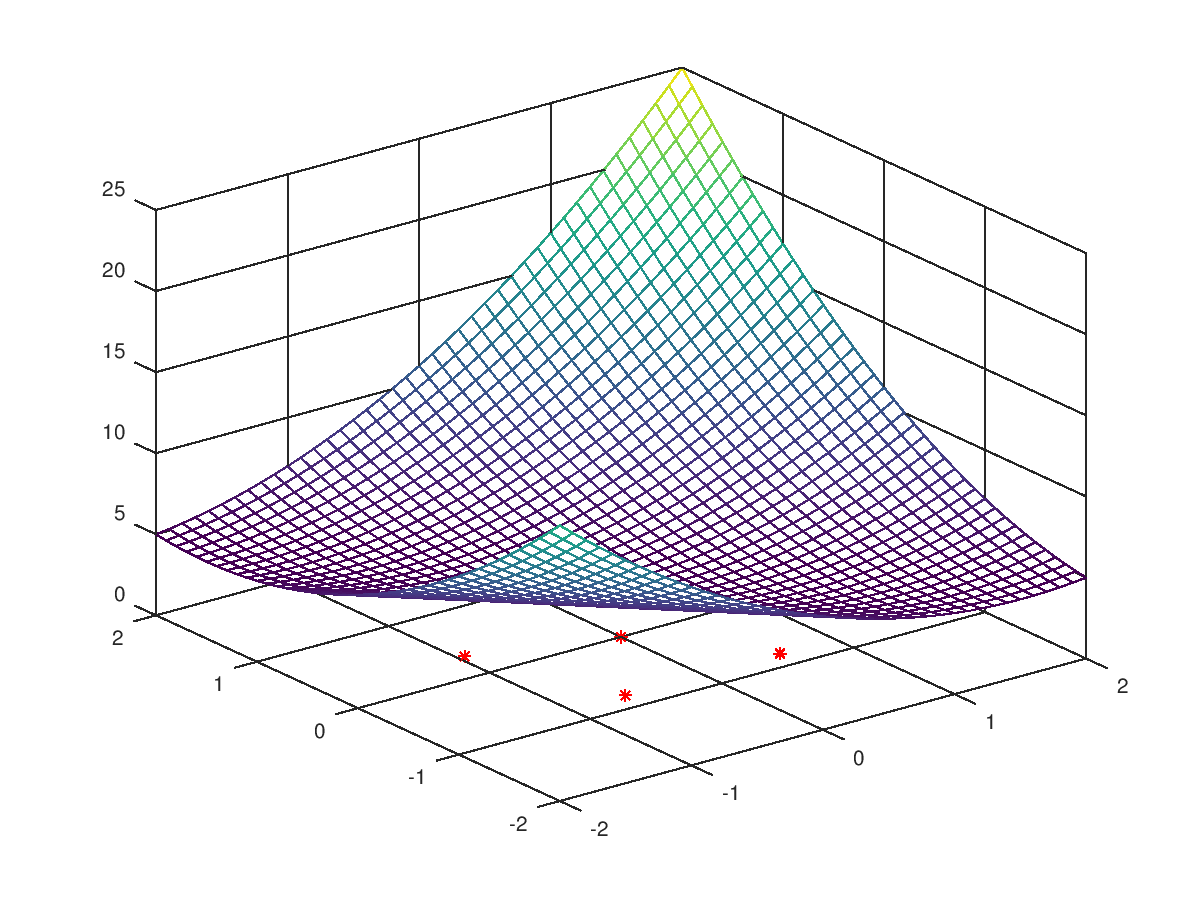
\includegraphics[width=200px]{images/poised_good.png}
    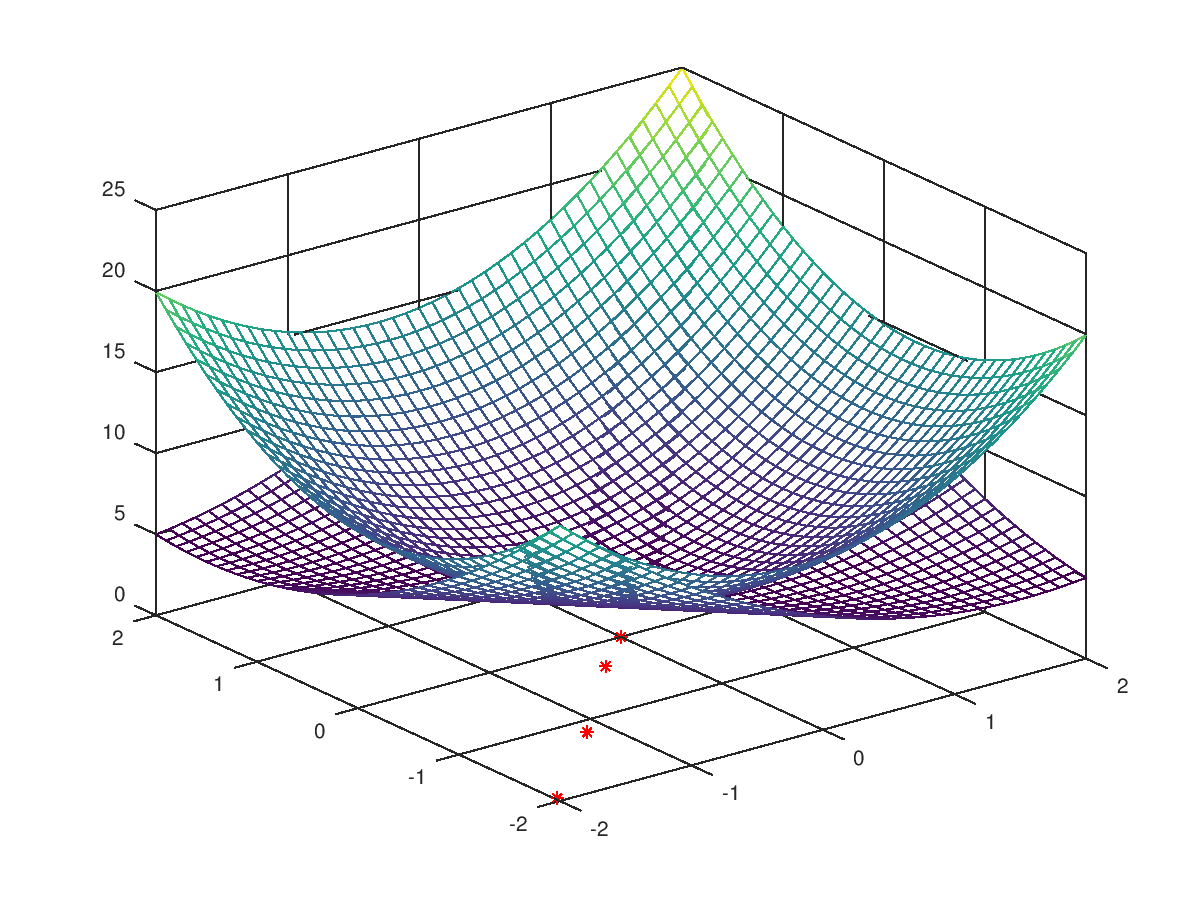
\includegraphics[width=200px]{images/poised_bad.png}
    \caption{
		Poised vs Ill poised.
		On the left, a well poised sample set is used and the model is indistinguishable from the true function.
		On the right, the sample set has poor geometry, and the model goes above the true function.
	}
    \label{pvip}
\end{figure}


A more detailed discussion can be found in \cite{doi:10.1080/10556780802409296}, but a step to ensure good geometry is required for convergence analysis although it may come at the expense of adding more function evaluations.

\subsubsection{Geometry Ensuring Algorithms}

Sample points are chosen by a geometry ensuring algorithm.
At any given time, the algorithm has evaluated 1 or more sample points.
Initially, only the starting point $x_0$ is evaluated, so that points must be added to the sample set.
Evaluated points within the trust region should be reused when possible, but the algorithm may have to replace some points to ensure a well poised set on the new trust region.
We call the algorithm that adds points, replacing where necessary, the \emph{model improvement algorithm}.
One classic such algorithm is presented in \cite{DUMMY:intro_book}.

The idea behind this algorithm is to perform an LU factorization with partial pivoting on the Vandermonde matrix.
As we have seen, this computes the basis for the Lagrange polynomials corresponding to $Y$.
However, when this LU factorization encounters a small pivot, the point corresponding to that row is replaced, improving the condition number of the Vandermonde matrix.

In practice, we first shift the sample set $Y$ by subtracting the current iterate and dividing by the trust region radius:
\begin{align}
\bar{Y} = [0, \frac{y^1 - y^0}{\Delta}, \ldots, \frac{y^p - y^0}{\Delta}]
\end{align}

At times, the algorithm will not have all $p+1$ points.
This can be because it is only given one point during initialization, or because points not within the trust region are removed.
Because the model improvement algorithm requires all $p+1$ points, we initialize $y^i = y^0$ for any $0 < i \le p$ corresponding to a missing point.
We choose a threshold $0 < \ximin < 1$, and follow \cref{model_improving_algorithm}:

\begin{algorithm}[H]
    \caption{Model Improvement Algorithm}
    \label{model_improving_algorithm}
    \begin{itemize}
        \item[\textbf{Step 0}] \textbf{(Initialization)} \\
            Initialize $i=1$.
            Given a non-empty set $Y$ of $p+1$ points. 
            Construct the Vandermonde matrix $V_{i,j} = \phi_j(\frac 1 {\Delta}(y^i - y^0))$.
			Initialize constant $\ximin > 0$.
        \item[\textbf{Step 1}] \textbf{(Pivot)} \\
            Swap row $i$ with row $i_{\max} = \arg \max_{j|j\ge i} V_{j,i} $
        
        \item[\textbf{Step 2}] \textbf{(Check threshold)} \begin{itemize}
                \item[] If $|V_{i,i}| < \ximin$ then select \label{next_point} $\hat y = \argmax_{t | \|t\|\le 1} |\phi_i(t)|$
                \item[] Replace row $i$ with $V_{i, j} \gets \phi_j(\hat y)$.
            \end{itemize}
        
        \item[\textbf{Step 3}] \textbf{(LU)} \begin{itemize}
                \item[] Set $V_i \gets \frac{1}{V_{i,i}} V_i$
                \item[] Set $V_{\bullet j} \gets V_{\bullet j} - V_{i,j} V_{\bullet j} \forall j=i \ldots p$
            \end{itemize}
            If $i = p$ then \textbf{Stop}, otherwise Set $i \gets i+1$ and go to Step 1
    \end{itemize}
\end{algorithm}


\subsection{Algorithm Components}


We will discuss several building blocks of the algorithm before going into the algorithm's detail.

\subsubsection{Criticality Measure}

In order to define stopping criteria for the algorithm, we introduce a criticality measure $\chi$ which goes to zero as the iterates approach a first order critical point.
When the criticality measure is small, we must also decrease the trust region radius.
Once this has reached a small enough threshold $\tau_{\chi}$ and the trust region is small enough ($\Delta_k < \tau_{\Delta}$), we can terminate the algorithm.
For now, our algorithm is designed to work with convex constraints, so we employ a classic criticality measure discussed in \cite{ConnGoulToin00} of

\begin{align}
\chik = \|\iteratek - \text{Proj}_{\feasiblek}(\iteratek- \nabla \modelk(\iteratek))\|
\end{align}

where $\feasiblek$ denotes the feasible region: $\feasiblek = \{x \in X | \modelconstrainti(x) \le 0 \quad \forall i \in \mathcal I \wedge c_i(x) = 0 \quad \forall i \in \mathcal E \}$.
This criticality measure measures how far the current is from satisfying the first order optimality conditions for $\iteratek$ to be a constrained minimum of $\modelk$.
When $ \lim_{k\to\infty} \chik = 0$, $\lim_{k\to\infty}\Delta_k = 0$, and $\lim_{k\to\infty}\iteratek = x^{\star}$, then we have that $x^{\star}$ also satisfies the first order optimality conditions of being a constrained minimum of $f$.

%we have $x = \text{Proj}_{\feasiblek}(x - \nabla \modelk(x))$ so that

We can compute $\chik$ as follows:
\begin{align}
\label{critical}
\trialk = \min_{s \in \feasiblek} \|\iteratek - \nabla \modelk(\iteratek) - s\|^2 \\
\chik = \|\iteratek - \trialk \|^2
\end{align}



% This remains large while there is feasible search space along a descent direction, but small otherwise or if the gradient goes to zero.

% Namely, when $ \chik(x) = 0$, we have $x = \text{Proj}_{\feasiblek}(x - \nabla \modelk(x))$ so that there is no decent direction along $\nabla \modelk(x)$ as it points away from the feasible region.
% As $\Delta_k$ gets smaller, we also have that $\modelk$ better represents $\nabla f$, so that $\nabla f$ will also either be zero or lie in the iterate's normal cone.

\subsubsection{Assessing Model Accuracy and Radius Management}

Each iteration that evaluates a trial point must also test the accuracy of the model functions.
To test the accuracy, we calculate a quantity
\begin{align}
\label{rho}
\rho_k = \frac{f(\iteratek) - f(\iteratek+\trialk)}{\modelk(\iteratek) - \modelk(\iteratek+\trialk)}
\end{align}
which measures the actual improvement over the predicted improvement.
A small $\rho_k$ implies the model functions are not sufficiently accurate.
Values of $\rho_k$ close to $1$ imply that the model accurately predicted the new objective value.
A large $\rho_k$ implies progress minimizing the objective although the model was not accurate.
This has been widely used within trust region frameworks such as \cite{Conn:2000:TM:357813} and within a derivative free context \cite{DUMMY:intro_book}.
The user supplies fixed constants $0 < \gammasm \le \gammabi \le 1$ as thresholds on $\rho_k$ and $0 < \omega_{\text{dec}} < 1 \le \omega_{\text{inc}}$ as decrement or increment factors to determine the trust region update policy.
The update policy frequently follows Step 4 within algorithm \cref{unconstrained_dfo} repeated within \cref{trust_region_update} for ease.

\begin{algorithm}[H]
    \caption{Trust Region Update Policy}
    \label{trust_region_update}
    \begin{itemize}
        \item[\textbf{Step 4}] \textbf{(Test for improvement)} \\
            Compute $\rho_k$ with \cref{rho} \begin{itemize}
                \item[] If $\rho_k < \gammasm$ then set $\iteratekpone \gets \iteratek$ (reject) and $\Delta_{k+1} \gets \omegadec\Delta_{k}$
                \item[] If $\rho_k \ge \gammasm$ and $\rho < \gammabi$ then set $\iteratekpone\gets\iteratek+\trialk$ (accept) and $\Delta_{k+1} \gets \omegadec\Delta_{k}$
                \item[] If $\rho_k \ge \gammabi$ and $\|\trialk\| = \Delta_{k}$ then set $\iteratekpone=\iteratek+\trialk$ (accept) and $\Delta_{k+1} \gets \omegainc\Delta_{k}$
                % and either increase the radius or decrease if $\nabla \modelk(\iteratek)$ is small
            \end{itemize}
            $k \gets k+1$ and go to Step 1.
    \end{itemize}
\end{algorithm}

\subsubsection{Sufficient Model Reduction}

To ensure sufficient reduction of the objective's model function during each iteration, we impose the following efficiency condition:
\begin{equation}
\label{efficiency}
\modelk(\iteratek) - \modelk(\iteratek + \trialk) \ge \kappa_f \chi_k \min\left\{ \frac{\chi_k}{1+\|\nabla^2 \modelk(\iteratek)\|}, \dk, 1 \right\}
\end{equation}
where $\kappa_f$ is a constant independent of $k$.
This is widely used within trust region frameworks such as \cite{Conejo:2013:GCT:2620806.2621814} and \cite{Conn:2000:TM:357813}.
It can be shown that the \emph{generalized Cauchy point} satisfies this condition \cite{Conn:2000:TM:357813}.



\section{The Algorithm}


\subsection{Algorithm Template}

We follow an algorithm template described in \cite{doi:10.1080/10556788.2015.1026968}, where variations of the algorithm have different choices of $ \sampletrk $ implemented in a \emph{ConstructTrustRegion} subroutine.
The different versions are described in the remainder of this section.

% HOW ABOUT JUST MAKE $\eta > 0$?


\begin{algorithm}[H]
    \caption{Always-feasible Constrained Derivative Free Algorithm}
    \label{constrained_dfo}
    \begin{itemize}
        \item[\textbf{Step 0}] \textbf{(Initialization)} \\
            Initialize tolerance constants
            $\tau_{\xi} \ge 0$,
            $\tau_{\Delta} \ge 0$,
            starting feasible ellipsoid $ \sampletrk $ containing initial iterate $x^{(0)} \in \domain$,
            initial radius $\Delta_0 > 0$,
            iteration counter $k=0$,
            $0 < \omegadec < 1 \le \omegainc$,
            $0 < \gammasm < \gammabi \le 1$,
            $\alpha > 0$,
            $0 < \Delta_0 < \Delta_{\text{max}} < \frac 1 2 diam(\domain)$,
            $k \gets 1$,
            $0 < \omegadec < 1 \le \omegainc$,
            $0 < \gammasm < \gammabi < 1$.
            
        \item[\textbf{Step 1}] \textbf{(Construct the model)} \\
            Ensure that the sample points are poised with respect to $ \sampletrk $ for \cref{accuracy} by calling \cref{model_improving_algorithm}.
            Construct $\modelk$ as described in \cref{reg} to construct $\modelk(x)$.
            
            If any point within $ \sampletrk $ is found to be infeasible, call \infeasiblesacred
            
            $ {T_{\text{interp}}^{(k+1)}} \gets $ \Call{ConstructTrustRegion}{$\Delta_k, x^{(k)}$}.
        
        \item[\textbf{Step 2}] \textbf{(Check stopping criteria)} \\
            Compute $\chi_k$ as in \cref{critical}. \begin{itemize}
                \item[] If $ \chik < \tau_{\xi} $ and $\dk <\tau_{\Delta}$ then return $\iteratek$ as the solution.
                \item[] Otherwise, if $\dk > \alpha \chik$ then 
                $\Delta_{k+1} \gets \omegadec \Delta_{k}$, 
                $x^{(k+1)} \gets \iteratek$,
                $k \gets k+1$ and go to Step 1.
            \end{itemize}
        
        \item[\textbf{Step 3}] \textbf{(Solve the trust region subproblem)} \\
			Compute the next trial point using \cref{linear_cut_trust_region}.
            
        \item[\textbf{Step 4}] \textbf{(Test for improvement)} \\
            Evaluate $f(\iteratek + \trialk)$ and evaluate $\rho_k$ as in \cref{rho} \begin{itemize}
                \item[] If $\rho_k < \gammasm$ then $\iteratekpone=\iteratek$ (reject) and $\Delta_{k+1} = \omegadec\Delta_{k}$
                \item[] If $\rho_k \ge \gammasm$ and $\rho < \gammabi$ then $\iteratekpone=\iteratek+\trialk$ (accept), $\Delta_{k+1} = \omegadec\Delta_{k}$
                \item[] If $\rho_k > \gammabi$ then $\iteratekpone=\iteratek+\trialk$ (accept), $\Delta_{k+1} = \omegainc\Delta_{k}$
                % and either increase the radius or decrease if $\nabla \modelk(\iteratek)$ is small
            \end{itemize}
            $k \gets k+1$ and go to Step 1.
    \end{itemize}
\end{algorithm}



The \emph{ConstructTrustRegion} works by constructing cones that buffer the inner trust region away from the constraints.
We would ideally construct the largest volume ellipsoid within the intersection of these cones.
This ellipse must be bounded by a constant of the trust region radius, and have a bounded condition number.
However, we have not completed a forumation of this problem.
Use have constructed a smaller cone, and found the center of an spherical inner trust region.




\subsection{Algorithm Modifications}
As can be seen from the differences within this algorithm and the classical algorithm, several modifactions had to be made in order to account for derivative free constraints.
We will discuss these modifications here.


\subsubsection{Criticality Measure}

The first change is our use of the criticality measure:
\begin{align*}
\feasiblek = \{x \in X | \; \modelconstrainti(x) \le 0 \quad \forall \; 1 \le i \le m \}, \quad
\chik = \|\iteratek - \text{Proj}_{\feasiblek}(\iteratek - \nabla \modelk(\iteratek))\|.
\end{align*}

With well behaved, known constraints, this projection could be strengthened to
\begin{align*}
{\mathcal F}^{(k)} = \{x \in X | \; c_i(x) \le 0 \quad \forall \; 1 \le i \le m \}, \quad
\chik = \|\iteratek - \text{Proj}_{{\mathcal F}^{(k)}}(\iteratek- \nabla \modelk(\iteratek))\|.
\end{align*}
In fact, this second definition is what is used within \cite{doi:10.1080/10556788.2015.1026968}.



\subsubsection{Trust Regions}
Our algorithm maintains two trust regions.
The outer trust region is an $L_1$ ball of radius $ \dk $ defined by
\begin{equation}
\label{trust_region}
\outertrk = B_{\infty}(\iteratek,\dk) = \{x\in \mathbb R^n | \; {\iteratek}_i - \dk \le x_i \le {\iteratek}_i + \dk \quad \forall 1\le i \le n\}.
\end{equation}

Note that the outer trust region may include infeasible points.
To ensure feasibility of all sample points, we construct an ellipsoidal inner trust region for sample points $ \sampletrk $  satisfying 
$\sampletrk \subset \outertrk \cap \feasiblek$ and $\iteratek \in \sampletrk $.
However, we do not want to limit the search for a new iterate to the same trust region we use to construct the model.
This means that within the trust region subproblem, we search over $\outertrk \cap \feasiblek$.

One convenience of this ellipsoidal trust region approach is that we can reuse classical methods for ensuring good geometry.
We can construct $\sampletrk$ to be ellipsoidal and use efficient algorithms within \cite{DUMMY:intro_book} to satisfy \cref{accuracy}.

The search trust region is used while selecting the next iterate:
\begin{align*}
\trialk = \argmin_{\trialk \in \outertrk \cap \feasiblek} \modelk(\iteratek + \trialk)
\end{align*}


The classical methods for ensuring good geometry require an optimization call to the model functions over a sphere.
This is no longer possible in the polyhedral trust region approach.
However, the bounds produced over the entire trust region may also be stronger than required as the models will only be used on the feasible region.
This may mean the geometric requirements can be reduced.
Looking again at the ill-poised set in \cref{aoip}, the set of nearly collinear sample points actually does appear to be accurate over a smaller trust region.


\begin{figure}[h]
    \centering
    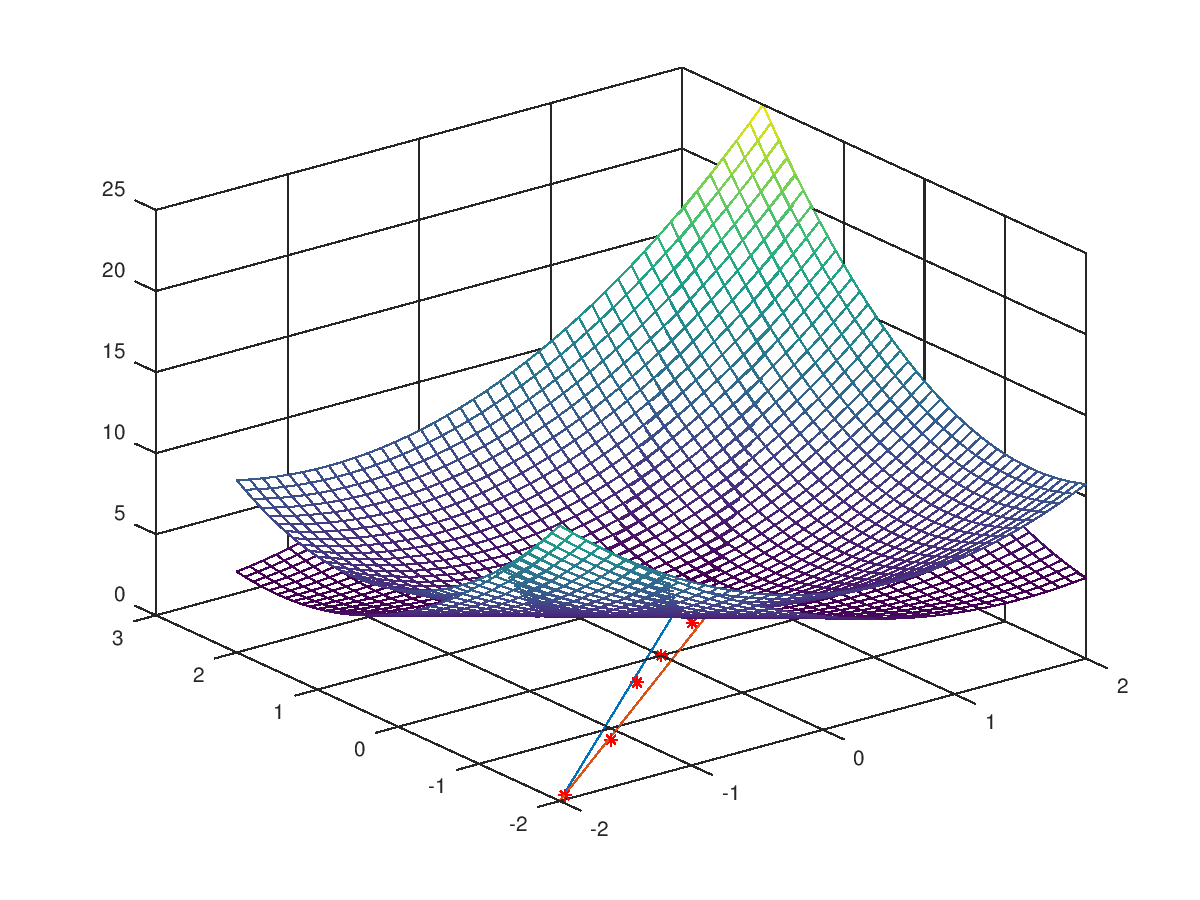
\includegraphics[width=200px]{images/poised_bad_but_good.png}
    \caption{Accurate model over thin trust region from illpoised set}
    \label{aoip}
\end{figure}



Another difficulty inherent in derivative free constraints is that a point expected to be feasible will prove infeasible upon evaluation.
This can happen in two different cases, 
\begin{itemize}
	\item While constructing the inner trust region, a sample point is infeasible.
	\item After solving the trust region subproblem, the trial point is infeasible.
\end{itemize}

\subsubsection{Infeasible Inner trust region}

When a sample point is infeasible, we can use previous feasible evaluations to create a new inner trust region.
Because we begin with an entire feasible ellipsoid, we know that the first sample set must be feasible.
This means that we will always have a set of poised, feasible points as well as the current iterate which is itself feasible.
Because the feasible region is convex, we are able to create a feasible ellipsoid within the convex hull of the previous sample points and the current iterate.
Note that the choice to use a feasible ellipsoid during the initialization could have been replaced with a poised sample set.
This is the \infeasiblesacred routine.


Namely, for a set of previous sample points $y^{(i)}$ and current iterate $\iteratek$, we can use the ellipse:

\begin{align*}
\Delta_{k+1} = \\
\innertrk = 
\end{align*}


We show that this step must only happen a finite number of times, because as the method of constructing the feasible inner trust region becomes accurate for small enough trust regions.


\subsubsection{Trust Region subproblem}

When the trial point is infeasible, we modify the trust region subproblem.
We add a linear constraint that ensures we do not attempt the same evaluation.

\begin{algorithm}[H]
    \caption{Trust Region Subproblem}
    \label{linear_cut_trust_region}
    \begin{itemize}
        \item[\textbf{Step 0}] \textbf{(Initialization)} \\
			Iteration counter $k = 0$ \\
            A set of infeasible evaluations $H_{\text{inf}} = \emptyset$ \\
            A set of feasible evaluations $H_{\text{feas}}$ of previous points that can be reused \\
			A samll tolerance $\epsilon \in (0, 1)$
            
        \item[\textbf{Step 1}] \textbf{(Minimize Modelled Constraints)} \\
            Compute
\begin{displaymath}
\begin{array}{cccccc}
s^{(k)} = \argmin_{s, v^{(j)}, b^{(j)}}	& \modelk(s) 	                         &       &                            				& 	\\
							& \left(u_{\text{fe}}^{(i)}\right)^T v^{(j)}     & \le   & b^{(j)}                     		& \quad \forall \; u_{\text{fe}}^{(i)} \in H_{\text{feas}}	\\
							& \left(u_{\text{infe}}^{(j)}\right)^T v^{(j)}      & \ge   & b^{(j)} + \epsilon \Delta_k   & \quad \forall \; u_{\text{infe}}^{(j)} \in H_{\text{inf}}  \\
							& \|v^{(i)}\|^2   & =     & 1                           									& \quad \forall \; 1 \le i \le |  H_{\text{inf}} | \\
							& s          & \in   & \sampletrk    														&	\\
\end{array}
\end{displaymath}
           
        \item[\textbf{Step 2}] \textbf{(Evaluate trial point)} \\
			\begin{itemize}
				\item[] If $s^{(k)}$ is defined and feasible, return $s^{(k)}$
				\item[] If $ s^{(k)} $ is not defined or $ s^{(k)} \in \sampletrk$, \textbf{fail}.
				\item[] Else $ s^{(k)} $ is defined and infeasible:
					$H_{\text{inf}} \gets H_{\text{inf}} \cup \{ s^{(k)} \} $, $k \gets k + 1$, Go to Step 1
			\end{itemize}
    \end{itemize}
\end{algorithm}



Note that this algorithm terminates in a finite number of steps.
By construction, all points added to $H_{\text{inf}}$ must have distance $\Delta  \epsilon_{\Delta}$ from other points within $H_{\text{inf}}$,
and there can be at most $\epsilon_{\Delta}^n$ such points in the outer trust region.

Also, note that the minimum value found by this algorithm is smaller than the minimum value atleast a distance $\epsilon \Delta_k$ from an infeasible point.



\subsection{Buffering Cones}

First, we will describe the buffering cones.
To ease the definition of these cones, we will use the following notation.


For all $1 \le i \le m$, $k = 1, \ldots$, define (\color{red} or assume \color{black}) the following whenever they exist:
\begin{align}
\alpha, \beta \in (0, 1) \label{def_alpha_beta} \\
\|\nabla c_i(x) - \nabla c_i(y)\| \le \lgi \|x - y\| \label{def_lipshitz} \\
\f = \{x \in \rn | \quad c_i(x) \le 0\quad \forall 1 \le i \le m \} \label{def_feasible} \\
\gik = \nabla m_{c_i}(\xk) \label{def_g} \\
\hgik = \frac{\gik}{\|\gik\|} \label{def_gk} \\
\zik = \xk - \frac{m_{c_i}(\xk)}{\|\gik\|}\hgik \label{def_z} \\
\wik = \xk + \left(1 - \alpha\dk^{\frac 1 2}\right)\left(\zik - \xk\right) \label{def_w} \\
\fik = \left\{x \in \rn | x = \wik + t s,t > 0, \|s\| = 1, -s^T\hgik \ge \beta \dk^{\frac 1 2 }\right\} \label{def_f} \\
\iik = \{1\le i \le m | \zik \in B_{\infty}(\xk, \dk) \} \label{def_i} \\
\huk = \max_{\{w \; | \; \|w\| = 1\}} \min_{1\le i\le m} w^T \hgik\label{def_hu} \\
\inf_{k}\min\{\sigma(\nabla c_{\mathcal I_k}(\xk)) \; | \; \sigma(\nabla c_{\mathcal I_k}(\xk)) > 0 \} \ge \epsilon_{\sigma} > 0\\
\end{align}


\subsubsection{Maximal Volume Ellipsoid}

Ideally, we would construct the maximum volume ellipsoid.


Given a set of vectors $v_i$ and scalars $0 < \beta_i < 1$ for $1\le i\le m$, define the set
\begin{align*}
P = \left\{x\bigg|\;-\frac{(x - v_i)^T}{\|x - v_i\|} \frac{v_i}{\|v_i\|} \ge \beta_i \; \forall 1 \le i \le m\right\}.
\end{align*}
(For the time being, assume that $v_i \ne 0$.)
We wish to choose a $Q$ and $c$ that maximizes the volume of the ellipsoid
\begin{align*}
E = \left\{x | (x - c)^TQ(x - c) \le r \right\}
\end{align*}
subject to $E \subseteq P$.


\subsubsection{A Feasible Sphere}

One simplification of this problem is to construct a feasible sphere.

To compute the maximum volume sphere, we can maximize the minimum distance from the center of any cone.
Thus, for some $\beta$, we wish to compute the projection of an arbitrary point $(t, y)$ and the second order cone: $\left\{ x \in \mathbb R^n | \quad x^Te_1 = \beta \|x\| \right\}$.

In general, if $x = (x_1, x')$, then
\begin{align*}
 \\
x^Te_1 = \beta \|x\| 
 \Longleftrightarrow x_1^2 = \beta^2 \|x_1e_1  + x - x_1 e_1\|^2 \\
 \Longleftrightarrow x_1^2 = \beta^2 \left(\|x_1e_1\|^2  + \|x - x_1 e_1\|^2\right) \\
 \Longleftrightarrow x_1^2 = \beta^2 \left(\|x_1e_1\|^2  + \|x - x_1 e_1\|^2\right) \\
 \Longleftrightarrow x_1^2 = \beta^2 \left(x_1^2  + \|{x'}\|^2 \right) \\
 \Longleftrightarrow (1 - \beta^2)x_1^2 = \beta^2 \|{x'}\|^2 \\
 \Longleftrightarrow \sqrt{\frac{1 - \beta^2}{ \beta^2}} x_1 = \|{x'}\|
\end{align*}

This means, that if we let $\beta' = \sqrt{\frac{1 - \beta^2}{\beta^2}}$, we have
\begin{align*}
\left\{ x \in \mathbb R^n | \quad x^Te_1 = \beta \|x\| \right\} = \left \{(s, x)\in \mathbb R^n | \quad\|x\| \le \beta' s \right\}.
\end{align*}

The projection gives the following optimization problem:
\begin{align*}
\min_{x \in \mathbb R^{n-1}, s \in \mathbb R} & \quad \frac 1 2 \|x - y\|^2 + \frac 1 2 (s - t)^2 \\
			& \quad \frac 1 2 \|x\|^2 = \frac 1 2 {\beta'}^2 s^2
\end{align*}
which gives us the Lagranian:
\begin{align*}
l(x, s, \lambda) = \frac 1 2 \|x - y \|^2 + \frac 1 2 \left(s - t\right)^2 - \lambda \frac 1 2 \left(\|x\|^2 - {\beta'}^2 s^2\right)
\end{align*}

After taking the gradient of the lagrangian, we find that for some $\lambda$:
\begin{align*}
x - y - \lambda x = 0, & \quad s - t + \lambda {\beta'}^2 s = 0 \\
x = \frac {y}{1 - \lambda}, & \quad s = \frac {t}{1 + \lambda {\beta'}^2 } \\
\end{align*}

We can substitute this into the constraint to solve for $\lambda$:
\begin{align*}
\|x\| = {\beta'} s \\
\left\|\frac {y}{1 - \lambda}\right\| = {\beta'} \frac {t}{1 + \lambda {\beta'}^2 } \\
\left(1 + \lambda {\beta'}^2\right) \left\|y\right\| = {\beta'}  {t} \left|1 - \lambda\right|\\
\end{align*}

\begin{align*}
\left\|y\right\| + {\beta'}^2\left\|y\right\|\lambda = t {\beta'} - t {\beta'} \lambda          &   \quad
\left\|y\right\| + {\beta'}^2\left\|y\right\|\lambda = t {\beta'} \lambda - t {\beta'}					\\
\left\|y\right\|-t {\beta'} +\left( {\beta'}^2\left\|y\right\| + t {\beta'} \right)\lambda = 0  &		\\
\lambda = \frac{t {\beta'} - \|y\|}{{\beta'}^2\|y\| + t {\beta'}}                               &		\\
\end{align*}


Substituting $\lambda$ to find $x$ and $s$:
\begin{align*}
x = \frac {y}{1 - \lambda} 																		
= \frac {y}{1 - \frac{t{\beta'} - \|y\|}{{\beta'}^2\|y\| + t{\beta'}}} 									
= \frac {y\left({\beta'}^2\|y\| + t{\beta'}\right)}{{\beta'}^2\|y\| + t{\beta'} - t{\beta'} + \|y\|} 			
= \frac {{\beta'}^2 + \frac{t{\beta'}}{\|y\|}}{1 + {\beta'}^2}y 											
\end{align*}

\begin{align*}
s = \frac {t}{1 + \lambda{\beta'}^2 } 
= \frac {t}{1 +\frac{t{\beta'} - \|y\|}{{\beta'}^2\|y\| + t{\beta'}}{\beta'}^2 } 
= \frac {t\left({\beta'}^2\|y\| + t{\beta'}\right)}{{\beta'}^2\|y\| + t{\beta'} + \left(t{\beta'} - \|y\|\right){\beta'}^2 } 
= \frac {{\beta'}\|y\| + t}{1 + {\beta'}^2 } 
\end{align*}


Thus, the projected point is
\begin{align*}
\left(\frac{{\beta'} \|y\| + t}{1 + {\beta'} ^ 2}, \frac{{\beta'} ^ 2 + t \frac {{\beta'}}{\|y\|}}{1 + {\beta'} ^ 2}y\right)
\end{align*}

with squared distance
\begin{align*}
\left(\frac{{\beta'} \|y\| + t}{1 + {\beta'} ^ 2} - t\right)^2 + \left\|\frac{{\beta'} ^ 2 + t \frac {{\beta'}}{\|y\|}}{1 + {\beta'} ^ 2}y - y\right\|^2
= \left(\frac{{\beta'} \|y\| + t}{1 + {\beta'} ^ 2} - \frac{t + t{\beta'} ^ 2}{1 + {\beta'} ^ 2}\right)^2 + \left(\frac{{\beta'} ^ 2 + t \frac {{\beta'}}{\|y\|}}{1 + {\beta'} ^ 2} - 1\right)^2\left\|y\right\|^2 \\
= \left(\frac{{\beta'} \|y\| - t{\beta'}^2}{1 + {\beta'} ^ 2}\right)^2 + \left(\frac{{\beta'} ^ 2 + t \frac {{\beta'}}{\|y\|} - 1 - {\beta'} ^ 2}{1 + {\beta'} ^ 2}\right)^2\left\|y\right\|^2 
= \left(\frac{{\beta'} \|y\| - t{\beta'}^2}{1 + {\beta'} ^ 2}\right)^2 + \left(\frac{t {\beta'} - \left\|y\right\|}{1 + {\beta'} ^ 2}\right)^2 \\
= \left(1 + {\beta'}^2\right)^{-2}\left[\left({\beta'}^2 \|y\|^2 - 2\beta' \|y\| t {\beta'}^2  + t^2 {\beta'}^4\right) + \left(t^2{\beta'}^2 - 2 t {\beta'} \|y\| + \|y\|^2\right) \right] \\
= \left(1 + {\beta'}^2\right)^{-2}\left[
\left(1 + {\beta'}^2\right)t^2{\beta'}^2 - 2t{\beta'}\left(1 + {\beta'}^2\right) \|y\| + \left(1 + {\beta'}^2\right)\|y\|^2
\right] \\
= \frac{\left(t \beta' - \|y\|\right)^2}{1 + {\beta'}^2}
\end{align*}

We wish to shift and rotate this from an arbitrary point $w^j$ going along a direction $-w^j$.
The rotation matrix for this rotation is 
\begin{align*}
R^j = 2 \frac{(e_1 + \hat w^j)(e_1 + \hat w^j)^T}{(e_1 + \hat w^j)^T(e_1 + \hat w^j)} - I  & \quad 1 \le j \le m \\
\end{align*}

so that the optimization problem becomes:
\begin{align*}
\max_{r \ge 0, c, t^j}	& r & \\
					& t^j = R^j({\hat w}^j - c) 																		& \quad 1 \le j \le m \\
					& \beta^2 \left(\beta' e_1^T t^j - \left\|t^j - e_1^T t^j\right\|\right)^2 \ge r			& \quad 1 \le j \le m \\
					& \left(\left(c - w^j\right)^T\hat w^j\right)^2 \ge \beta^2 \|c - w^j\|^2											& \quad 1 \le j \le m \\
\end{align*}


\subsubsection{Feasible Ellipsoid}

However, we have been able to construct one feasible ellipse that satisfies our requirements.

If we define
\begin{align}
\theta^{\text{min}}_k = \min_{i \in \mathcal I} (-\hgik)^T \huk \label{def_theta_k_min} \\
\theta^{\text{max}}_k = \max_{i \in \mathcal I} (-\hgik)^T \huk \label{def_theta_k_max} \\
\theta^{\text{min}} = \liminf_{k\to\infty} \theta^{\text{min}}_k \label{def_theta_min} \\
\theta^{\text{max}} = \limsup_{k\to\infty} \theta^{\text{max}}_k \label{def_theta_max} \\
\bs = \sqrt{ 1 - (\theta^{\text{max}}_k)^2} \label{def_bs} \\
\bsk = \beta\dk^{\frac 1 2} \theta^{\text{max}}_k + \sqrt{(1 - \dk\beta^2)\left(1 - (\theta^{\text{max}}_k) ^2\right)} \label{def_bs_k} \\
\fcki = \{x \in \rn | \quad x = \xk + ts, t > 0, \|s\| = 1, s^T\huk \ge \bsk \} \label{feasible_cone} \\
0 < g_{\text{low}} \le \|\gik\| \le g_{\text{hi}} \label{def_g_bounds} \\
0 < h_{\text{low}} \le \|\nabla^2m_{c_i}(x)\| \le h_{\text{hi}} \label{def_h_bounds} \\
f_e(\delta, r, \theta; x) = (x - \delta e_1)^T\bigg(\begin{bmatrix}
1 & \boldsymbol0^T \\
\boldsymbol 0 & \frac{\theta^2}{1 - \theta^2} \boldsymbol I \\
\end{bmatrix}\bigg)(x - \delta e_1) - \frac 1 2 r^2 \label{def_ellipse_function} \\
R = 2\frac{(e_1 + \huk)(e_1 + \huk)^T}{(e_1 + \huk)^T(e_1 + \huk)} - \boldsymbol I \label{def_rotation} \\
E_k = \{x \in \rn | f_e\left(\frac 1 2 \dk, \frac 1 2 \dk, \bsk; R(x - \xk)\right) \le 0\} \label{def_ellipse_k} \\
\nabla c_i(\xk) = \nabla m_{c_i}(\xk) + \epsilon_{g}\dk^2\nu \label{def_lambda_poised} \\
\end{align}

We will show that $E_k$ is such an ellipsoid.



\begin{theorem}
Let $\theta^{\text{min}}$ be as defined as in \cref{def_theta_min}.
Then $\theta^{\text{min}} > 0.$
\end{theorem}

\begin{proof}
We assume that $\nabla c_{\mathcal I_k}(\xk)$ has full rank.
Let $n_k$ be the number of rows in $\nabla c_{\mathcal I_k}(\xk)$, and $d = \min \{ n, n_k \}$.
Give $\nabla m_{c_{\mathcal I_k}}(\xk)$ and $\nabla c_{\mathcal I_k}(\xk)$ their singular value decompositions
\begin{align*}
\nabla m_{c_{\mathcal I_k}}(\xk) = U\Sigma V^T, \quad
\nabla c_{\mathcal I_k}(\xk) = \hat U \hat \Sigma \hat V^T
\end{align*}
where $U, \hat U$ are orthonormal $n_k \times d$ matrices; $\Sigma, \hat \Sigma$ are diagonal $d \times d$ matrices; and $V, \hat V$ are orthonormal $d \times n$ matrices.
Note that because of \cref{def_lambda_poised}, if $\|\cdot\|_{\mathcal F}$ is the Frebenious norm, then
\begin{align*}
\|\nabla c(\xk) - \nabla m_{c_{\mathcal I_k}}(\xk)\|_{\mathcal F}^2 \le n_k \left(\epsilon_g \dk^2\right)^2
\Longrightarrow \|\nabla c(\xk) - \nabla m_{c_{\mathcal I_k}}(\xk)\|_{\mathcal F} \le \sqrt{n_k} \epsilon_g \dk^2.
\end{align*}
Each element $\hat \Sigma$ is greater than $\epsilon_{\sigma}$, so because $\dk \to 0$ we have that for sufficiently large $k$, each element of $s$ of $\Sigma$ satisfies $s > \frac 1 2 \epsilon_{\sigma}$.

First, we compute
\begin{align*}
\nabla \hat m_{c_{\mathcal I_k} }(\xk) \uk = -\nabla\hat m_{c_{\mathcal I_k} }(\xk) \nabla\hat m_{c_{\mathcal I_k} }(\xk)^{-1} e
= -(U\Sigma V^T)(V\Sigma^{\dagger} U^T)e
= -e 
\end{align*}
and
\begin{align*}
\|\uk\| = \|V\Sigma^{\dagger} U^Te\|  
\le \frac 1 {\sigma_{\text{min}}\left(\nabla \hat m_{c_{\mathcal I_k}}(\xk)\right)}.
\end{align*}

Then we can see that
\begin{align*}
(-\gik)^T\huk = -\frac{\|\gik\|}{\|\uk\|}(\hgik)^T\uk = \frac{\|\gik\|}{\|\uk\|} \ge g_{\text{low}} \sigma_{\text{min}}\left(\nabla \hat m_{c_{\mathcal I_k}}(\xk)\right) \ge \frac 1 2 g_{\text{low}}\epsilon_{\sigma}. \\
\end{align*}

% -A^T(AA^T)^{-1}Ae = \\


\end{proof}




\begin{theorem}
\label{cone_subset_cone}
Given $u^1, u^2 \in \rn$, $\|u^1\| = \|u^2\|= 1$, $\beta >0$, with ${u^1}^Tu^2 \ge \beta$ define
\begin{align*}
B = \{x\in\rn | {u^2}^Tx \ge \beta\|x\|\}, \quad
S = \left\{x\in\rn \bigg| {u^1}^Tx \ge \left(\beta {u^1}^Tu^2 + \sqrt{(1 - \beta^2)\left(1 - ({u^2}^Tu^1)^2\right)}\right)\|x\| \right\}. 
\end{align*}
Then, $S \subseteq B$.
\end{theorem}


\begin{proof}
Let 
\begin{align*}
x^{\star} = \beta u^2 + \sqrt{\frac{1 - \beta^2}{1 - ({u^2}^Tu^1)^2}} (u^1 - {u^2}^Tu^1 u^2 )
\end{align*} and for a contradiction, let $y \in \rn$ be such that $y \not \in B$ and $y \in S$ and define $\hat y = \frac{y}{\|y\|}$.
Then
\begin{align*}
\hat y \in \left\{x \in \rn | {u^2}^Tx < \beta, {u^1}^Tx \ge \beta {u^1}^Tu^2 + \sqrt{(1 - \beta^2)\left(1 - ({u^2}^Tu^1)^2\right)} \right\}.
\end{align*}

Note that
\begin{align}
{u^1}^Tx^{\star} &=& {u^1}^T\left(\beta u^2 + \sqrt{\frac{1 - \beta^2}{1 - ({u^2}^Tu^1)^2}} (u^1 - {u^2}^Tu^1 u^2 )\right) = 
\beta {u^1}^Tu^2 + \sqrt{(1 - \beta^2)\left(1 - ({u^2}^Tu^1)^2\right)} \\
{u^2}^Tx^{\star} &=& {u^2}^T\left(\beta u^2 + \sqrt{\frac{1 - \beta^2}{1 - ({u^2}^Tu^1)^2}} (u^1 - {u^2}^Tu^1 u^2 )\right) = 
\beta + \sqrt{\frac{1 - \beta^2}{1 - ({u^2}^Tu^1)^2}} ({u^2}^Tu^1 - {u^2}^Tu^1 ) = \beta.
\end{align}
That means
\begin{align}
{u^1}^T\hat y = {u^1}^T\left(x^{\star} + \hat y - x^{\star}\right) = \beta {u^1}^Tu^2 + \sqrt{(1 - \beta^2)\left(1 - ({u^2}^Tu^1)^2\right)} + {u^1}^T\left(\hat y - x^{\star}\right) \\
\ge \beta {u^1}^Tu^2 + \sqrt{(1 - \beta^2)\left(1 - ({u^2}^Tu^1)^2\right)} 
\Longrightarrow {u^1}^T\left(\hat y - x^{\star}\right) \ge 0 \\
{u^2}^T\hat y = {u^2}^T\left(x^{\star} + \hat y - x^{\star}\right) = \beta + {u^2}^T\left(\hat y - x^{\star}\right) < \beta
\Longrightarrow {u^2}^T\left(\hat y - x^{\star}\right) < 0. \label{the_difference_is_nonzero}
\end{align}

From these two equations, we not only know that $\left(\hat y - x^{\star}\right) \ne 0$, but
\begin{align*}
{\left(\hat y - x^{\star}\right)}^Tx^{\star} = 
\left(\beta {\left(\hat y - x^{\star}\right)}^Tu^2 + \sqrt{\frac{1 - \beta^2}{1 - ({u^2}^Tu^1)^2}} \left({\left(\hat y - x^{\star}\right)}^Tu^1 - {u^2}^Tu^1 {\left(\hat y - x^{\star}\right)}^Tu^2 \right)\right) > 0
\end{align*}
as ${u^1}^Tu^2 \ge \beta \Longrightarrow {u^2}^Tu^1\sqrt{\frac{1 - \beta^2}{1 - ({u^2}^Tu^1)^2}} \ge \beta$.
However, this is a contradiction as
\begin{align*}
1 = \|\hat y\| = \|x^{\star} + \hat y - x^{\star}\| > \|x^{\star}\| = 1
\end{align*}
and there is no such $y$.
Thus, any $y \in\rn$ with $y \in S$ must also have $y \in B$.
\end{proof}






\begin{theorem}
If 
\begin{align}
z^{(i, k)} \in B_{\infty}(\xk, \dk)) \label{z_is_active} \\
M \ge \sup_{x \in B_{\infty}(\xk, \dk)} \frac 1 2 \nabla^2 c_i(x) \label{m_bounds} \\
\text{and} \quad \dk \le \min\left\{
1,
\left(\frac{\alpha g_{\text{low}}}{M \sqrt{n} + \epsilon_g}\right)^2,
\left(\frac{\beta}{2\epsilon_{g}}g_{\text{low}}\right)^{\frac 2 3},
\left[\frac {g_{\text{low}} \beta} {2M\sqrt{n}\left(1 + \frac {\lgi} M \right)} \right]^2
\right\}, \label{delta_is_small_enough}
\end{align} then
\begin{align*}
c_i(x) \le 0 \quad \forall x \in \fik \cap B_{\infty}(\xk, \dk).
\end{align*}

\end{theorem}

\begin{proof}

Let 
\begin{align}
y = \wik + ts \in \fik \cap B_{\infty}(\xk, \dk) \label{t_is_bounded}
\end{align}
with $t > 0, \|s\| = 1, -s^T\hgik \ge \beta \dk^{\frac 1 2}$.
Because the model $m_{c_i}$ is fully quadratic, we know that there exists a $\nu\in\rn$ such that \cref{def_lambda_poised} holds:
\begin{align*}
\nabla c_i(\xk) = \nabla m_{c_i}(\xk) + \epsilon_{g}\dk^2\nu.
\end{align*}

First, we will show that $c(\wik) \le 0$.
For simplicity, we use \cref{def_cg}, \cref{def_gk}, \cref{def_z}, and \cref{def_w} to compute
\begin{align}
\wik - \xk & = & \xk + \left(1 - \alpha \dk^{\frac 1 2 }\right)\left(\zik - \xk\right) - \xk 
= \left(1 - \alpha \dk^{\frac 1 2 }\right)\left(\zik - \xk\right) \\
& = &  \left(1 - \alpha \dk^{\frac 1 2 }\right)\left(\xk - \frac{c_i(\xk)}{\|\gik\|^2}\gik - \xk\right) 
= \left(1 - \alpha \dk^{\frac 1 2 }\right)\frac{-c_i(\xk)}{\|\gik\|^2}\gik. \label{simple_computation}
\end{align}

Also, note by \cref{delta_is_small_enough}, \cref{def_alpha_beta} that both
\begin{align*}
\dk \le \left(\frac{\alpha \|\gik\|}{M \sqrt{n} + \epsilon_g}\right)^2 \Longrightarrow 
M \sqrt{n}\dk^{\frac 1 2} + \epsilon_g \dk^{\frac 1 2} \le \alpha \|\gik\| \quad \text{and} \quad
0 < 1 - \alpha \dk^{\frac 3 2 } < 1.
\end{align*}
We can combine these and \cref{z_is_active} to find 
\begin{align*}
M \sqrt{n}\dk^{\frac 1 2}\left(1 - \alpha \dk^{\frac 3 2 }\right)^2  + \epsilon_g \dk^{\frac 3 2} \left(1 - \alpha \dk^{\frac 3 2 }\right) \le M \sqrt{n}\dk^{\frac 1 2} + \epsilon_g \dk^{\frac 1 2} & \le & \alpha \|\gik\| \\
\Longrightarrow -\alpha \dk^{\frac 1 2 }\|\gik\| + M \left(1 - \alpha \dk^{\frac 3 2 }\right)^2 \sqrt{n}\dk+ \epsilon_g \dk^2 \left(1 - \alpha \dk^{\frac 3 2 }\right) & \le &  0 \\
\Longrightarrow -\alpha \dk^{\frac 1 2 }\|\gik\|\left(-\frac{c_i(\xk)}{\|\gik\|}\right) + M \left(1 - \alpha \dk^{\frac 3 2 }\right)^2 \left(-\frac{c_i(\xk)}{\|\gik\|}\right)^2+ \epsilon_g \dk^2 \left(1 - \alpha \dk^{\frac 3 2 }\right)\left(-\frac{c_i(\xk)}{\|\gik\|}\right) & \le& 0.
\end{align*}

However, we also know by \cref{m_bounds}, \cref{simple_computation} and the Mean Value Theorem, that
\begin{align*}
0 &\ge& \alpha \dk^{\frac 1 2 } c_i(\xk) + M \frac {c_i(\xk)^2}{\|\gik\|^2}\left(1 - \alpha \dk^{\frac 1 2 }\right)^2 + \epsilon_g \dk^2 \left(1 - \alpha \dk^{\frac 1 2 }\right)\frac{-c_i(\xk)}{\|\gik\|} & \\
&\ge& \alpha \dk^{\frac 1 2 } c_i(\xk) + M \frac {c_i(\xk)^2}{\|\gik\|^2}\left(1 - \alpha \dk^{\frac 1 2 }\right)^2 + \epsilon_g \dk^2 \left(1 - \alpha \dk^{\frac 1 2 }\right)\frac{-c_i(\xk)}{\|\gik\|^2}\nu^T\gik & \\
&=& c_i(\xk)\left[1 - \left(1 - \alpha \dk^{\frac 1 2 }\right)\right] + M \frac {c_i(\xk)^2}{\|\gik\|^2}\left(1 - \alpha \dk^{\frac 1 2 }\right)^2 + \epsilon_g \dk^2\nu^T \left(\wik - \xk\right) & \\
&& + \epsilon_g \dk^2\nu^T \left(\wik - \xk\right) & \\
&=& c_i(\xk) + \left(\gik\right)^T\left(1 - \alpha \dk^{\frac 1 2 }\right)\frac{-c_i(\xk)}{\|\gik\|^2}\gik + M \left\|\left(1 - \alpha \dk^{\frac 1 2 }\right)\frac{-c_i(\xk)}{\|\gik\|^2}\gik\right\|^2 & \\
&=& c_i(\xk) + \left(\gik\right)^T\left(\wik - \xk\right)+ M \left\|\wik - \xk\right\|^2  + \epsilon_g \dk^2\nu^T \left(\wik - \xk\right) & \\
 & = & c_i(\xk) + \nabla c_i(\xk)^T\left(\wik - \xk \right) + M \left\|\wik - \xk\right\|^2 \ge c_i(\wik). &
\end{align*}


Also, by \cref{def_f} we know that $-s^T \hgik \ge \beta \dk^{\frac 1 2}$ where $\|s\| = 1$, and by \cref{def_g_bounds}, \cref{def_gk}, \cref{def_lambda_poised}, and our assumption \cref{delta_is_small_enough}, we know

% \Longrightarrow \dk^{\frac 3 2} \le \frac{\beta}{2\epsilon_{g}}g_{\text{low}}
% \Longrightarrow -s^T\gik \ge \frac 1 2 g_{\text{low}} \beta \dk^{\frac 1 2} + \epsilon_{g}\dk^2\nu^T s \\
\begin{align}
\dk \le \left(\frac{\beta}{2\epsilon_{g}}g_{\text{low}}\right)^{\frac 2 3} 
\Longrightarrow \dk^{\frac 3 2} \le \frac{\beta}{\epsilon_{g}}\left(g_{\text{low}} - \frac 1 2 g_{\text{low}}\right)
\Longrightarrow \frac{\epsilon_{g}}{\beta} \dk^{\frac 3 2} \le \|\gik\| - \frac 1 2 g_{\text{low}} \nonumber \\
\Longrightarrow -\|\gik\|s^T\hgik \ge \|\gik\|\beta\dk^{\frac 1 2} \ge \frac 1 2 g_{\text{low}} \beta \dk^{\frac 1 2} + \epsilon_{g}\dk^2 
\Longrightarrow -s^T\gik \ge \frac 1 2 g_{\text{low}} \beta \dk^{\frac 1 2} + \epsilon_{g}\dk^2|\nu^T s| \nonumber \\ 
\Longrightarrow -s^T\left(\gik + \epsilon_{g}\dk^2\nu\right) \ge \frac 1 2 g_{\text{low}} \beta \dk^{\frac 1 2} 
\Longrightarrow -s^T\nabla c_i(\xk) \ge \frac 1 2 g_{\text{low}} \beta \dk^{\frac 1 2}. \label{nsc_pos}
\end{align}

% So that if $\xk + ts \in B_{\infty}(\xk, \dk)$, then 

We also know by \cref{delta_is_small_enough} that
% \Longrightarrow \dk^{\frac 1 2} \le \frac {g_{\text{low}} \beta} {2M\sqrt{n}\left(1 + \frac {\lgi} M \right)}
\begin{align}
\dk \le \left[\frac {g_{\text{low}} \beta} {2M\sqrt{n}\left(1 + \frac {\lgi} M \right)} \right]^2 
\Longrightarrow \sqrt{n}\left(1 + \frac {\lgi} M \right) \dk^{\frac 1 2} \le \frac 1 {2M} g_{\text{low}} \beta \nonumber \\
\Longrightarrow \sqrt{n}\left(1 + \frac {\lgi} M \right) \dk \le \frac 1 {2M} g_{\text{low}} \beta \dk^{\frac 1 2}
\Longrightarrow \sqrt{n} \dk \le -\frac 1 M \sqrt{n}\dk \lgi + \frac 1 {2M} g_{\text{low}} \beta \dk^{\frac 1 2} \label{eqn2}
\end{align}
which implies by \cref{def_g_bounds}, \cref{t_is_bounded}, \cref{nsc_pos}, \cref{eqn2}

% t \le -\frac 1 M \left( \sqrt{n}\dk L_g + \nabla c_i(\xk)^Ts\right) \\
\begin{align}
t 
\le \sqrt{n} \dk 
\le -\frac 1 M \sqrt{n}\dk \lgi + \frac 1 {2M} g_{\text{low}} \beta \dk^{\frac 1 2} 
\le -\frac 1 M \sqrt{n}\dk \lgi -\frac 1 M \nabla c_i(\xk)^Ts \nonumber \\
\Longrightarrow \sqrt{n}\dk \lgi + \nabla c_i(\xk)^Ts + M t \le 0. \label{eqn3}
\end{align}

From there, we can conclude with \cref{def_lipshitz}, \cref{z_is_active}, \cref{eqn3}
\begin{align*}
c_i(y) = c_i(\wik + ts) \le c_i(\wik) + t\nabla c_i(\wik)^Ts + M t^2 \\
\le t \left(\nabla c_i(\wik)^Ts - \nabla c_i(\xk)^Ts + \nabla c_i(\xk)^Ts + M t\right) \\
\le t \left(\lgi\|\wik - \xk\| + \nabla c_i(\xk)^Ts + M t\right) \\
\le t \left(\sqrt{n}\dk \lgi + \nabla c_i(\xk)^Ts + M t\right) \le 0.
\end{align*}

% Thus, the entire cone $\fik$ is feasible with respect to the linearization of the constraint $c_i$ for sufficiently small $\dk$.
% \begin{align*}
% c_i(\xk + ts) \le c_i(\xk) + t\nabla c_i(\xk)^Ts + Mt^2 \le t(\nabla c_i(\xk)^Ts + Mt) \le 0.\\
% \end{align*}


\end{proof}



\begin{theorem}
We have that $\cap_{i \in \iik} \fik \cap B_{\infty}(\xk, \dk) \subseteq \f$ 
\end{theorem}

\begin{proof}
This follows directly from $x \in \fik \cap B_{\infty}(\xk, \dk) \Longrightarrow c_i(x) \le 0$.
\end{proof}



\section{Convergence Discussion}
\label{convergence_discussion}

If the tolerances $\tau_{\chi} = 0$ and $\tau_{\Delta} = 0$ are set to zero, the algorithm presented here is nearly a particular implementation of the algorithm presented in \cite{doi:10.1080/10556788.2015.1026968}.
Thus, five hypothesis are required for the convergence analysis:

\begin{itemize}
\item[H0] The trial point during each iterate satisfies the efficiency condition \cref{efficiency}.
\item[H1] The function $f$ is differentiable and its gradient $\nabla f$ is Lipschitz continuous over $\domain$.
\item[H2] The function $f$ is bounded below over $\domain$.
\item[H3] The Hessian's of $f$ are uniformly bounded at each iterate.
\item[H4] The accuracy condition \cref{accuracy}.
\end{itemize}

Hypothesis H1, H2, and H3 are kept as assumptions within our algorithm.
Hypothesis 0 is satisfied by the Generalized Cauchy Point \cite{Conn:2000:TM:357813} if we set $\searchtrk = \outertrk \cap \feasible$ as discussed in \cref{search_a_lot}.
As discussed in \cref{ellipsoidal_lambda}, Hypothesis H4 is satisfied by letting $\sampletrk$ have an ellipsoidal shape as discussed within \cref{bluepill} as long as the condition number of $\qk$ is bounded.

However, we must ensure that we are always able to find a feasible ellipsoid.
Although it is not always possible to find a feasible ellipsoid that contains the current iterate,
we can find a feasible ellipse that needs only be scaled by a constant to do so.
It is shown in \cite{Billups_Larson_2013} that a lambda poised set over a sphere remains lambda poised over a larger sphere (with a larger lambda).


\subsection{Poisedness over Ellipsoidal Trust Regions}

As long as \emph{ConstructTrustRegion} selects an ellipsoidal $ \sampletrk $, we ensure of a stronger version of \cref{accuracy}.
Namely, we will show \cref{ellipsoidal_lambda} that 
\[
    \|\modelk(x) - \nabla f(x) \| \le \kappa_g \Delta_{k} \quad \forall x \in \sampletrk.
\]
If we also choose our trial point with \cref{search_a_little}, we have no guarantee of satisfying the efficiency condition \cref{efficiency} because $\Delta_k$ is the outer trust region radius.
However, the model will likely be more accurate over this region.

It is possible to show $\Lambda$-poisedness for an ellipsoidal region with a change of variables to the ball centered around the origin.
We wish to construct a model for $f(x)$ in the ellipsoidal region
$\ellipsek = \{x \in \mathbb R^n | (x - c)^T\qk(x - c) \le 1\}$ for some symmetric, positive definite
$\qk \in \mathbb R^{n\times n}$ and some center $c \in \mathbb R^n$.
We can give $\qk$ its eigen-decomposition $\qk = L D^2 L^T$, where $L^TL = I$ and $D$ is a diagonal matrix with nonnegative entries.
If we let $\delta = \max_{x\in \ellipsek}\|x-c\|$, then the transformation $T(x) = \delta DL^T(x - c)$ maps $ \ellipsek $ to the $\delta$ ball $\{u = T(x) \in \mathbb R^n \; | \; \|u\| \le \delta\}$.
Conversely, $ T^{-1}(u) = \frac 1 {\delta} LD^{-1}u + c$ maps the $\delta$ ball to the ellipsoidal region $ \ellipsek $.

% \cref{fully_quadratic}

\begin{theorem}
Let $T$ and $\delta$ be as defined above, and let $\hat m_f(u)$ be a model of the shifted objective $\hat f(u) = f(T^{-1}(u))$ in the $\delta$ ball such that
there exist constants $\kappa_{ef}, \kappa_{eg}, \kappa_{eh} > 0$ such that for all $\{u \in R^n | \;\|u\| \le \delta \}$, we have
% for all $u \in B(0 ; \delta)$ we have the following error bounds:
\begin{align*}
|\hat m_f(u) - \hat f(u)| \le \kappa_{ef} \delta^3\\
\|\nabla \hat m_f(u) - \nabla \hat f(u)\| \le \kappa_{eg}\delta^2\\
\|\nabla^2 \hat m_f(u) - \nabla^2 \hat f(u)\| \le \kappa_{eh}\delta.
\end{align*}

Then, with
\begin{align*}
\kappa_{ef}' = \kappa_{ef} \\
\kappa_{eg}' = \kappa_{eg}\sqrt{\kappa(\qk)} \\
\kappa_{eh}' = \kappa_{eh}\kappa(\qk),
\end{align*}
we have that for all $x \in \ellipsek$,
the model function $m_f(x) = \hat m_f(T(x))$ will satisfy
\begin{align*}
| m(x) - f(x)| \le \kappa_{ef}'\delta^3 \\
\|\nabla  m(x) - \nabla  f(x)\| \le \kappa_{eg}'\delta^2 \\
\|\nabla^2 m(x) - \nabla^2 f(x)\| \le \kappa_{eh}'\delta.
\end{align*}
\end{theorem}

\begin{proof}

% Notice  that for all $x\in \ellipsek$ we have 
% \begin{align*}
% \|x-c\| \le \delta \\
% \|T(x-c)\| \le \delta \\
% \end{align*}
% so that $\frac{\|T(x-c)\|}{\|x-c\|} \le 

We know that $\delta = \frac 1 {\sqrt{\lambda_{\text{min}}(\qk)}} = \frac 1 {\min_{i} D_{i, i}}$.
This means,
\begin{align*}
\kappa(\qk) = \kappa(D^2) = \frac{\max_{i}D_{i,i}^2}{\min_{i}D_{i,i}^2} = \delta^2 \max_{i}D_{i,i}^2 = \delta^2 \|D\|^2 \\
\|D\| = \frac 1 {\delta} \sqrt{\kappa(\qk)} \le \frac{\kappa_{\lambda}}{\delta}.
\end{align*}

Also, $\delta \le \dk$ as the ellipse is constructed within the outer trust region.

Then, we have for all $\{u = T(x) \; | \; \|u\| \le \delta \} \Leftrightarrow x \in \ellipsek$

\begin{align*}
 | m_f(x) - f(x)| = |\hat m(u) - \hat f(u)| \le \kappa_{ef}'\dk^3.
\end{align*}

Similarily, for the gradient we find:

\begin{align*}
\| \nabla m_f(x) - \nabla f(x)\| = \delta\left\|DL^T\left(\nabla\hat m_f(u) - \nabla \hat f(u)\right)\right\| \le \delta \|DL^T\|\|\nabla \hat m_f(u) - \nabla \hat f(u)\| \le \sqrt{\kappa(\qk)}\kappa_{eg} \delta^2 \\
\end{align*}

Finally, we show that for the Hessian:

\begin{align*}
\| \nabla^2 m_f(x) - \nabla^2 f(x)\| = \delta^2\left\|DL^T\left(\nabla\hat m_f(u) - \nabla \hat f(u)\right)LD^T\right\| \le \delta^2 \|D\|^2\|\nabla \hat m_f(u) - \nabla \hat f(u)\| \le \kappa(\qk)\kappa_{eh} \delta \\
\end{align*}


\end{proof}

This shows that in order to have strongly quadratic model functions, we need only bound the condition number of $\qk$.
For the purposes of a convergence proof, we need only satisfy the weaker accuracy condition \cref{accuracy}.
Notice that in practice the model functions do not need to be mapped to the $\delta$ ball, because $\Lambda$-poisedness is scale invariant \cite{DUMMY:intro_book}.
The implications of this proof are discussed futher in the convergence discussion \cref{convergence_discussion}.




\begin{theorem}
For sufficiently small $\dk$, the set $\fcki \subseteq \fik$ for all $1\le i \le m$.
\end{theorem}


\begin{proof}
Fix some $1\le i \le m$.
Letting $\dk \le 1$, we see that $\xk \in \fik$:
\begin{align*}
\xk = \xk + \left(1 - \alpha\dk^{\frac 1 2}\right)(\zik - \xk) - \left(1 - \alpha\dk^{\frac 1 2}\right)(\zik - \xk) \\
\end{align*}
where
\begin{align*}
\frac{-\left(1 - \alpha\dk^{\frac 1 2}\right)(\zik - \xk)}{\left\|-\left(1 - \alpha\dk^{\frac 1 2}\right)(\zik - \xk)\right\|}^T\hgik = 1 \ge \beta\\
\end{align*}

% = -\frac{m_{c_i}(\xk)}{\|\gik\|}\frac{\|\gik\|}{m_{c_i}(\xk)}

Now, let $\dk$ be sufficiently small that $-(\huk)^T\hgik \ge \beta\dk^{\frac 1 2}$.
This is possible, because $ -(\huk)^T\hgik \ge \theta^{\text{min}}_k \ge \theta^{\text{min}} > 0$.

Then
\begin{align*}
\left\{s\quad | \quad s^T(-\hgik)\ge\dk^{\frac 1 2}\beta\|s\| \right\}  \subseteq \left\{s\quad | \quad s^T\huk\ge\beta^{\star}\|s\| \right\}
\end{align*}
by \cref{cone_subset_cone} with $u^1 \gets \hat u$, $u^2 \gets -\hgik$, $\beta \gets \beta \dk^{\frac 1 2 }$ because:
\begin{align*}
\left(-\beta\dk^{\frac 1 2}(\huk)^T\hgik + \sqrt{(1 - \dk\beta^2)\left(1 - \left((\hgik)^T\hat u^{(k)}\right)^2\right)}\right) \\
\le \max_i \left(-\beta\dk^{\frac 1 2}(\huk)^T{\hgik} + \sqrt{(1 - \dk\beta^2)\left(1 - \left((\hgik)^T\huk\right)^2\right)}\right) \\
\le \beta\dk^{\frac 1 2} \max_i\{-(\huk)^T\hgik\} + \sqrt{(1 - \dk\beta^2)\left(1 - \left((\max_i(-\hgik)^T\huk\right)^2\right)} \\
= \beta\dk^{\frac 1 2} \theta^{\text{max}}_k + \sqrt{(1 - \dk\beta^2)\left(1 - (\theta^{\text{max}}_k) ^2\right)} = \beta^{\star}
\end{align*}
Thus, $\fcki \subseteq \fik$.
\end{proof}

\begin{theorem}
For sufficiently small $\dk$, $\fcki \ne \emptyset$.
\end{theorem}
\begin{proof}
As $\dk \to 0$, $\bsk \to \sqrt{1 - (\theta^{\text{max}}_k) ^2} \ge \bs > 0$.
% Also, the ray $\xk + t \huk$ is within this cone.
\end{proof}



\begin{theorem}
\label{ellipse_in_cone}
Let $r \le \delta$.
Then $\{x \in \rn | f_e(\delta, r, \theta; x) \le 0\} \subseteq \{tx\in\rn| e_1^T x \ge \theta,\|x\|=1, t>0\}$.
\end{theorem}


\begin{proof}
Let $x$ be such that $f_e(\delta, r, \theta, x) \le 0$.
First, note that
\begin{align*}
(e_1^Tx - \frac 1 2 \delta )^2\ge 0\\
\Longrightarrow (e_1^Tx)^2 + e_1^Tx\delta  - \frac 1 4 \delta^2 \ge 0\\
\Longrightarrow 0 \le 2(e_1^Tx)^2 + 2e_1^Tx\delta  - \frac 1 2 \delta^2\\
\Longrightarrow \frac 1 2 \delta^2 - (e_1^Tx)^2 + 2e_1^Tx\delta - \delta^2 \le (e_1^Tx)^2 \\
\Longrightarrow \frac 1 2 \delta^2 - \left((e_1^Tx)^2 - 2e_1^Tx\delta + \delta^2\right) \le (e_1^Tx)^2 \\
\Longrightarrow \frac 1 2 \delta^2 - (e_1^Tx - \delta)^2 \le (e_1^Tx)^2.
\end{align*}

We use this inequality to show:
\begin{align*}
f_e(\delta, r, \theta, x) \le 0 \\
\Longrightarrow (x - \delta e_1)^T\bigg(\begin{bmatrix}
1 & \boldsymbol0^T \\
\boldsymbol 0 & \frac{\theta^2}{1 - \theta^2} \boldsymbol I \\
\end{bmatrix}\bigg)(x - \delta e_1) \le \frac 1 2 r^2 \\
\Longrightarrow (e_1^Txe_1 + (x - e_1^Txe_1) - \delta e_1)^T\bigg(\begin{bmatrix}
1 & \boldsymbol0^T \\
\boldsymbol 0 & \frac{\theta^2}{1 - \theta^2} \boldsymbol I \\
\end{bmatrix}\bigg)(e_1^Txe_1 + (x - e_1^Txe_1) - \delta e_1) \le \frac 1 2 r^2 \\
\Longrightarrow
(e_1^Tx - \delta)^2 + \frac{\theta^2}{1 - \theta^2}\|x - e_1^Tx e_1\|^2 \le \frac 1 2 r^2 \\
\Longrightarrow
(e_1^Tx - \delta)^2 + \frac{\theta^2}{1 - \theta^2}(\|x\|^2 - (e_1^Tx)^2) \le \frac 1 2 \delta^2 \\
\Longrightarrow\frac{\theta^2}{1 - \theta^2}(\|x\|^2 - (e_1^Tx)^2) \le \frac 1 2 \delta^2 - (e_1^Tx - \delta)^2\\
\Longrightarrow\|x\|^2 - (e_1^Tx)^2 \le \frac{1 - \theta^2}{\theta^2}(e_1^Tx)^2 \\
\Longrightarrow\|x\|^2 \le \frac 1 {\theta^2}(e_1^Tx)^2 \\
\Longrightarrow e_1^T\frac{x}{\|x\|} \ge \theta.
\end{align*}
\end{proof}

\begin{theorem}
\label{ellipse_fits}
We have that $f_e(\delta, \sqrt{2}\delta, \theta; 0) = 0$ and $f_e(\delta, \delta, \theta; (1 + \frac{1}{\sqrt{2}}) \delta e_1) = 0$
\end{theorem}
\begin{proof}

We have
\begin{align*}
f_e(\delta, \sqrt{2}\delta, \theta; 0) =(0 - \delta e_1)^T\bigg(\begin{bmatrix}
1 & \boldsymbol0^T \\
\boldsymbol 0 & \frac{\theta^2}{1 - \theta^2} \boldsymbol I \\
\end{bmatrix}\bigg)(0 - \delta e_1) - \frac 1 2 (\sqrt 2 \delta)^2
=\delta^2 - \delta^2 = 0\\
\end{align*}
and
\begin{align*}
f_e(\delta, \delta, \theta; (1 + \frac{1}{\sqrt{2}}) \delta e_1) =\frac {\delta}{\sqrt{2}}e_1^T\bigg(\begin{bmatrix}
1 & \boldsymbol0^T \\
\boldsymbol 0 & \frac{\theta^2}{1 - \theta^2} \boldsymbol I \\
\end{bmatrix}\bigg)\frac {\delta}{\sqrt{2}}e_1 - \frac 1 2 \delta^2
=\frac 1 2 \delta^2 - \frac 1 2 \delta^2 = 0.\\
\end{align*}

\end{proof}

\begin{theorem}
For sufficiently small $\dk$, the ellipse $E_k \subseteq \f$ has a bounded condition number, and its major axis is atleast $\frac 1 2 \dk$
\end{theorem}

\begin{proof}
Note that the condition number is given by
\begin{align*}
\frac{\max\{1, \frac{\bs^2}{1 - \bs^2}\}}{\min\{1, \frac{\bs^2}{1 - \bs^2}\}}
\end{align*}
because the condition number of a matrix is not affected by rotations.

We have already shown that the cone $\fcki \cap B_{\infty}(\xk, \dk) \subset \f$.
By construction, the ellipse has been shifted to put $\xk$ at the origin and rotated by $R$ to put $\hat u$ along the x-axis.
Thus, by \cref{ellipse_in_cone}, we know that $E_k \subseteq \fcki$.
We know that $t_k > \dk$ because it measures the distance from $\xk$ to some point on the boundary of $B_{\infty}(\xk, \dk)$.
Also, we know from \cref{ellipse_fits} that the ellipse can be scaled by $2$ to include $\xk$, and extends by $\frac 1 2 \dk$ along $\huk$.
Finally, we know that it does not travel more than $\dk$ from $\xk$, so that it is contained within $B_{\infty}(\xk, \dk)$.
\end{proof}



\subsection{Convergence of projections}

\color{red}


\begin{align*}
C = \{ x \in X | Gx\le g, Dx = g \} \\
C' = \{ x \in X | G'x\le g', D'x = g' \} \\
\|G - G'\| \le \epsilon \\
\|g - g'\| \le \epsilon \\
\|D - D'\| \le \epsilon \\
\|d - d'\| \le \epsilon \\
\xo = \argmin_{x\in C}\|x\|^2 \\
\xo' = \argmin_{x\in C'}\|x\|^2 \\
G = \begin{bmatrix}A \\ B\end{bmatrix} \\
g = \begin{bmatrix}a \\ b\end{bmatrix} \\
N = \begin{bmatrix}B \\ D\end{bmatrix}\\
N' = \begin{bmatrix}B' \\ D'\end{bmatrix}\\
\text{rank}(N) = r \\
\text{rank}(N') = r \\
\end{align*}



\begin{theorem}
There exist positive constants $\epsilon_0$ and $c$ such that for all $\epsilon \le \epsilon_0$,  one has $\|\xo - \xo'\| \le c \sqrt{\epsilon}$.
\end{theorem}



\color{black}



\subsection{Modified Proof}


We will define:

%\rk = \frac{f(\iteratek) - f(\iteratek + \trialk)}{\modelk(\iteratek) - \modelk(\iteratek + \trialk)} \\
%\modelk(\iteratek + \trialk) = f(\iteratek) + (\gk)^T \trialk + \frac 1 2 \trialk^T \hk \trialk \\
%\chik = \|P_{\Omega}(\iteratek - \gk) - \iteratek \| \\

\begin{align*}
S = \{k \in \ints | \rk > \eta \} \\
\bar{S} = \{k \in \ints | \rk \ge \eta_1 \} \\
c = \frac{L + \kappa_{g} + \frac {\beta} 2}{\kappa_f} \\
c_0 = L + \kappa_{g} + \frac {\beta} 2 \\
\mathcal K = \big \{ k \in \ints | \dk \le \min \{ \frac {\chik}{\beta}, \frac{1-\eta_1}{\chik}c, \oalpha \chik, 1 \} \big \}
\end{align*}



\subsubsection{$\mathcal K \subset \bar{S}$}
\begin{theorem}
Suppose that Hypothesis H1 and H2 hold. If $k \in \mathcal K$, then $k \in \bar{S}$.
\end{theorem}
 
\begin{proof}

By the Mean Value Theorem, there exists a $t_k \in (0, 1)$ such that
\begin{align*}
f(\iteratek + \trialk) = f(\iteratek) + \grad(\iteratek + t_k\trialk)^T\trialk
\end{align*}

By H1, H3, H4,
\begin{align*}
|f(\iteratek) - f(\iteratek + \trialk) - (\modelk(\iteratek) - \modelk(\iteratek + \trialk)| \\
= |-(\grad(\iteratek + t_k\trialk) - \gk)^T\trialk + \frac 1 2 (\trialk)^T \hk \trialk| \\
\le (\| \grad(\iteratek + t_k\trialk) - \grad(\iteratek) \| + \| \grad(\iteratek)-\gk \|) \|\trialk\| + \frac 1 2 \|\trialk\|^2\|\hk\| \\
\le (t_k L \|\trialk\| + \kappa_{g}\dk) \|\trialk\| + \frac 1 2 \beta \|\trialk\|^2
\end{align*}

Since $\| \trialk \| \le \dk$ and $t_k \in (0, 1)$ we have that
\begin{align}
|f(\iteratek) - f(\iteratek + \trialk) - (\modelk(\iteratek) + \modelk(\iteratek + \trialk)| \le c_0 \dk^2
\end{align}

By the definition of $\mathcal K$, for every $k \in \mathcal K$ we have that $\dk \le \oalpha \chik$ and consequently $\chik > 0$.
By the efficiency condition, this means that $\modelk(\iteratek) - \modelk(\iteratek + \trialk) \ne 0$.
Then,
\begin{align*}
|\rk - 1| = \bigg |\frac{f(\iteratek) - f(\iteratek + \trialk) - (\modelk(\iteratek) - \modelk(\iteratek + \trialk)}{\modelk(\iteratek) - \modelk(\iteratek + \trialk)} \bigg | \\
\le \frac {c_0 \dk^2} {\kappa_f \chik \min\{\frac{\chik}{\beta}, \dk, 1\}} \\
= \frac {c \dk^2} {\chik \min\{\frac{\chik}{\beta}, \dk, 1\}}
\end{align*}

We also know that 
\begin{align*}
\dk = \min\{\frac {\chik} {\beta}, \dk, 1 \} \\
\frac {c \dk}{\chik} \le 1 - \eta_1
\end{align*}
so that
\begin{align*}
|\rk - 1| \le 1 - \eta_1 \\
\Longrightarrow \rk \ge \eta_1
\end{align*}
so that $k \in \bar{S}$.


\end{proof}



\subsubsection{$\Delta_k \to 0$}
\begin{theorem}
Suppose Hypothesis H2, H3. Then the sequence $(\dk)$ converges to zero.
\end{theorem}
 
\begin{proof}

Suppose that $\bar{S}$ is finite. Then there exists $k_0 \in \ints$ such that for all $k \ge  k_0$, $\dkpo \le \omegadec \dk$.
Thus, $(\dk)$ converges to zero.
From now on $\bar{S}$ is infinite.
For any $k \in \bar{S}$, we know $\dk \le \oalpha \chik$ using $H3$ we have
\begin{align*}
f(\iteratek) -  f(\xkpo) \ge \eta_1 \big (\modelk(\iteratek) - \modelk(\iteratek + \trialk)\big ) \ge \eta_1 \kappa_f \chik \min\{\frac{\chik}{\beta}, \dk, 1\}\\
f(\iteratek) - f(\xkpo) \ge \eta_1\kappa_f\frac{\dk}{\oalpha}\min\{\frac{\dk}{\oalpha \beta}, \dk, 1\}
\end{align*}
Because $f(\iteratek)$ is nonincreasing, the left hand side goes to zero.
Thus,
\begin{align}
\lim_{k \in \bar{S}} \dk = 0
\end{align}


Consider the set
$\mathcal U = \{ k \in \ints | k \not \in \bar S \}$.
If $\mathcal U$ is finite, then $\lim_{k\to\infty}\dk = 0$.
Otherwise, consider $k \in \mathcal U$ and define $\l_k$ to be the last index in $\bar S$ before $k$.
Then $l_k$ is well-defined for all large $k$  and $\dk \le \omegainc \Delta_{l_k}$ which implies that
\begin{align}
\lim_{k \in \mathcal U } \dk \le \omegainc \lim_{k \in \mathcal U} \Delta_{l_k} = \omegainc \lim_{l_k \in \bar{S}} \Delta_{l_k}
\end{align}

so that $\lim_{k \in \mathcal U} \dk = 0$.

\end{proof}




\subsubsection{$\chik \to 0$ Part 1}
\begin{theorem}
Suppose that Hypothesis H1, H4. Then $\liminf_{k\to\infty} \chik = 0$.
\end{theorem}
 
\begin{proof}
Suppose for a contradiction that there exists a constants $\epsilon > 0$ and an integer $K > 0$ such that for $\chik \ge \epsilon$ for each $k \ge K$.
Take $ \tilde \Delta = \min \{\frac{\epsilon}{\beta}, \frac{(1 - \eta_1)c}{\epsilon}, \oalpha \epsilon, 1\}$.
Consider $k \ge K$.
If $\dk \le \tilde \Delta$, then $k \in \mathcal K$.
Then $k \in \bar S$ and thus $\dkpo \ge \dk$.
Therefore, the trust region radius can only decrease if $\Delta > \tilde \Delta$, and in this case $\dkpo = \omegadec\dk > \omegadec \tilde \Delta$.
Therefore, one can see that for all $k \ge K$
\begin{align}
\dk \ge \min\{\omegadec \tilde \Delta, \dk \}
\end{align}
which is a contradiction.
\end{proof}



\subsubsection{$\chik \to 0$ Part 2}
\begin{theorem}
Suppose that H1 to H4 and $\eta > 0$. Then $\lim_{k\to\infty}\chik=0$.
\end{theorem}

\begin{proof}
Suppose for a contradiction that for some $\epsilon > 0$ the set $\int ' = \{k \in \ints | \chik \ge \epsilon \}$
is finite.

Because $\lim_{k\to\infty}\Delta_k\to 0$, there exists a $k_0 \in \ints$ such that for all $k \ge k_0$,

\begin{align*}
\dk \le \min\{\frac{\epsilon}{\beta}, \frac{(1-\eta_1)\epsilon}{c}, \oalpha\chik, 1\}.
\end{align*}

Then if $k \in \ints '$ with $k \ge k_0$:

\begin{align*}
\dk \le \min\{\frac{\chik}{\beta}, \frac{(1-\eta_1)\chik}{c}, \oalpha\chik, 1\}
\end{align*}

and therefore $k \in \bar S \subset S$.

Given $k \in \ints'$ with $k\ge k_0$, consider $l_k$ the first index such that $l_k > k$ and $\chi_{l_k} \le \frac{\epsilon} 2$.
The existence of $l_k$ is ensured by lemma 3.3.
This means that $\chik - \chi_{l_k} \ge \frac {\epsilon} 2 $.
Using the definition of $\chik$, the triangle inequality and the contraction property of projections, we have that

\begin{align*}
\frac{\epsilon}{2} \le \|P_{\Omega}(\iteratek - \gk) - \iteratek\| - \|P_{\Omega}(x^{(l_k)} - g^{(l_k)}) - x^{(l_k)}\| \\
\le \|P_{\Omega}(\iteratek - \gk) - \iteratek - P_{\Omega}(x^{(l_k)} - g^{(l_k)}) + x^{(l_k)}\| \\
\le 2\|\iteratek - x^{(l_k)}\| + \|\gk - g^{(l_k)}\| \\
=   2\|\iteratek - x^{(l_k)}\| + \|\gk - \grad(\iteratek) + \grad(\iteratek) - \grad(x^{(l_k)}) + \grad(x^{(l_k)}) - g^{(l_k)}\| \\
\le 2\|\iteratek - x^{(l_k)}\| + \|\gk - \grad(\iteratek)\| + \|\grad(\iteratek) - \grad(x^{(l_k)})\| + \|\grad(x^{(l_k)}) - g^{(l_k)}\|.
\end{align*}

So that
\begin{align}
\frac{\epsilon} 2 \le (2 + L) \|\iteratek - x^{(l_k)}\| + \kappa_{g}(\dk + \Delta_{l_k}).
\end{align}

Consider $C_k = \{i \in S | k \le i < l_k\}$.
Note that because $k \in S$, so $C_k \ne \varnothing $.
For each $i \in C_k$, using the fact that $i \in S$, and H3, we conclude that 

\begin{align}
f(x^{(i)}) - f(x^{(i+1)}) \ge \eta\big ( \modelk(x^{(i)}) - \modelk(x^{(i)} + s^{(i)}) \big ) \ge \eta \kappa_f \chi_i \min\{\frac{\chi_{i}}{\beta}, \Delta_i, 1\} 
\end{align}

By the definition of $l_k$, we have that $\chi_i > \frac{\epsilon}{2}$ for all $i \in C_k$.
As $i \ge k$, $\Delta_i \le \frac{\epsilon}{\beta}$ and $\Delta_i \le 1$.
Therefore,
\begin{align}
\frac{\Delta_i}{2} \le \frac{\epsilon}{2\beta} \le \frac{\pi_i}{\beta}.
\end{align}

It follows that
\begin{align}
f(x^{(i)}) - f(x^{(i+1)}) > \frac{\eta \kappa_f \epsilon \Delta_i}{4}
\end{align}

and hence
\begin{align}
\Delta_i < \frac{4}{\eta \kappa_f \epsilon} \big ( f(x^{(i)}) - f(x^{(i+1)})\big ).
\end{align}

Meanwhile,
\begin{align}
\|x^{(i)} - x^{(l_k)}\| \le \sum_{i \in C_k}\|x^{(i)} - x^{(i+1)}\| \le \sum_{i \in C_k} \Delta_i
\end{align}

so that

\begin{align}
\|x^{(i)} - x^{(l_k)}\| < \frac{4}{\eta \kappa_f \epsilon} \big ( f(x^{(i)}) - f(x^{(i+1)})\big ).
\end{align}

We also know that $(f(\iteratek))$ is bounded below, and since it is nonincreasing, $f(\iteratek)  - f(x^{(l_k)}) \to 0$.
Therefore $(\|\iteratek - x^{(l_k)}\|)_{k \in \ints '}$ converges to zero.

\end{proof}

\subsubsection{Convergence}

\begin{theorem}
Suppose that H1 to H4 hold.

If $\eta = 0$, then
\begin{align}
\liminf_{k\to\infty} \|P_{\Omega}(\iteratek - \grad(\iteratek)) - \iteratek \| = 0.
\end{align}

If $\eta > 0$, then
\begin{align}
\lim_{k\to\infty} \|P_{\Omega}(\iteratek - \grad(\iteratek)) - \iteratek \| = 0.
\end{align}

\end{theorem}

\begin{proof}
By the triangle inequality, the contraction property of projections and H4, we have that

\begin{align*}
\|P_{\Omega}(\iteratek - \grad(\iteratek)) - \iteratek \| = \|P_{\Omega}(\iteratek - \grad(\iteratek)) - P_{\Omega}(\iteratek - \gk) + P_{\Omega}(\iteratek - \gk) - \iteratek\| \\
\le \|P_{\Omega}(\iteratek - \grad(\iteratek)) - P_{\Omega}(\iteratek - \gk)\| + \|P_{\Omega}(\iteratek - \gk) - \iteratek\| \\
\le \|\grad(\iteratek) - \gk\| + \|P_{\Omega}(\iteratek - \gk) - \iteratek\| \\
\le \kappa_{g} \Delta_k + \chik
\end{align*}

\end{proof}
 
\newpage

\appendix

\section{Table of Notation}
\begin{longtable}{| p{.20\textwidth} | p{.80\textwidth} |}
$\domain$ & is the domain \\
$\real$ & is the real numbers \\
$f$ & is the objective function \\
$f_{\text{min}}$ & is a lower bound on the objective function \\
$\beta$ & is a bound on the hessian of the model functions \\
$\modelk$ & is a model function of the objective at iteration $k$ \\
$c_i$ & are the constraints $\forall i \in \mathcal{I} \cup \mathcal{E} $ \\
$\modelconstrainti$ & is the model of constraint $i$ at iteration $k$ \\
$\modelconstraint$ & is the model of the vector valued constraint function at iterate $k$ \\
$\mathcal{I}$ & is the index set of the inequality constraints \\
$\mathcal{E}$ & is the index set of the equality constraints \\
$e_i$ & is the unit vector \\
$\phi_i$ & is a basis vector \\
$Y$ & is the set of sample points \\
$V$ & is a vander mode matrix \\
$y^i$ & is a sample point \\
$d$ & is the dimension of the space of model functions \\
$\lambda_i$ & are the weights of a linear combination \\
$\alpha_i$ & are the coefficients of a model function on its basis polynomials \\
$\phi_i$ & are basis polynomials \\
$p-1$ & is the size of the sample set \\
$l_i$ & is a lagrange polynomial \\
$\Lambda$ & is a constant bounding the poisedness of a sample set \\
$\kappa_{ef},\kappa_{eg},\kappa_{eh}$ & are constants used to bound the model's error \\
$\kappa_{f}$ & is a constant in the efficiency condition \\
$\kappa_{g}$ & is a constant in the accuracy condition \\
$\iteratek$ & is the current iterate in iteration $k$\\
$\trialk$ & is the trial point in iteration $k$ \\
$\chik$ & is the criticality measure in iteration $k$ \\
$\outertrk$ & is the outer trust region in iteration $k$ \\
$\feasible$ & is the feasible region \\
$\feasiblek$ & is the feasible region during iteration $k$ \\
% $\innerfritr$ & is the feasible region intersect the inner trust region \\
$\outerfritr$ & is the feasible region intersect the outer trust region \\
$s$ & is the decision variable within the trust region subproblem \\
$B_k(c; \Delta)$ & is the ball of radius $\Delta$ centered at point $c$ in the $k$ norm\\
& $B_k(c;\Delta) = \{ x \in \mathbb{R}^n : \| x - c\|_k \le \Delta \}$ \\
$\Delta$ & is the trust region radius \\
$\Delta_k$ & is the outer trust region radius in iteration $k$ \\
$\rho$ & measures actual improvement over the predicted improvement \\
$\gamma_1, \gamma_2$ &  are bounds on $\rho$ \\
$\omega_{\text{dec}}, \omega_{\text{inc}}$ & are scalars used to manipulate the trust region radius \\
$\tau$ & is a tolerance \\
$\mathcal{F}^k$ & is the feasible region \\
$f^k$ & is the function value \\
$g^k$ & is the gradient of the model \\
$A$ & is the jacobian of the constraint model functions \\
$\xi_{\text{min}}$ & is a tolerance within the LU pivoting algorithm \\
$T$ & is an affine transformation that brings the trust region back to the origin \\
$Q$ & is the semi-definite matrix defining the affine transformation $T$ \\
$L$ & is a cholesky factorization of $Q$ \\
$L$ & is the Lipschitz constant of $f$ \\
$\mu^k$ & is the center of the ellipse \\
$\ellipsek$ is the ellipse during iteration $k$ \\
$\pi$ & is a scaling factor while finding the ellipse \\
$d$ & are the differences between the center of the ellipse and where the ellipse intersect the constraints? \\
$M$ & is an upper bound \\
$P$ & is a polyhedron \\
$\delta_{i,j}$ & is the kronecker delta function, $\delta_{i,i} = 1$, $\delta_{i,j} = 0$ if $i\ne j$ \\
$\tau_{\xi}$ & is a threshold for the criticallity measure \\
$\tau_{\Delta}$ & is a threshold for the trust region radius
\label{tab:TableOfNotation}
\end{longtable}

\newpage


\bibliography{bibliography}
\bibliographystyle{ieeetr}

\end{document}


